\chapter{Muonic papers}

\begin{itemize}
\item multipole expansion of arbitrary nuclear potential
\item Introduce magnetic dipole and electric quadrupole hyperfine splitting in the Furry picture
\item introduce vacuum polarization corrections (Uehl, Quad-Uehl, WK, KS)
\item Describe usage of modified wave functions (Uehl+WK+KS)
\item Describe g factor correction for bound muon due to Uehl+KS (our PRD)
\item Describe modification of matrix elements with Quad-Uehl
\item Introduce dynamic hyperfine structure
\item Describe calculations of second order terms
\item Description of transition probabilities with hyperfine states
\end{itemize} 


\section{Introduction}
A muon is a charged elementary particle, which is in many aspects similar to the electron, in particular, it has the same electric charge, but it is ${\approx}\,{200}$ times heavier than the electron~\cite{codata}. When coming close to an atom, a muon can be captured by the nucleus and form a hydrogen-like muonic ion, which is typically also surrounded by the atomic electrons. This atomic system is commonly referred to as a muonic atom. The lifetime of the muon is big enough to be considered stable in the structure calculations of these muonic bound states. Muonic atomic systems feature strong dependence on nuclear parameters and therefore can provide information about atomic nuclei \cite{Wheeler1949}. This triggered interest in precise knowledge of the level structure of muonic atoms \cite{BorieRinker1982,Devons1995}. Due to the muon's high mass, it is located much closer to the nucleus; and, especially for heavy nuclei, this results in big nuclear size effects and a strong dependence of the muon bound state energies on the nuclear charge and current distributions, as well as large relativistic effects.

A combination of the knowledge about the level structure and experiments measuring the transition energies in muonic atoms enabled the determination of nuclear parameters like charge radii \cite{Piller1990,Schaller1980}, quadrupole moments \cite{Dey1979}, and magnetic HFS constants \cite{Ruetschi1984}. One of the most precise measurements to date is the determination of the nuclear root-mean-square radius of $^{208}$Pb on a $0.2\%$ level~\cite{Bergem1988}.

Recent measurements on muonic hydrogen renewed the interest in muonic atoms, revealing a disagreement between the values for the proton charge radius extracted from muonic and electronic systems \cite{Pohl2010}. This allows the assumption that there can be unidentified effects in muonic systems, and triggered detailed theoretical investigation of muonic hydrogen und light muonic atoms, e.g., Refs \cite{indelicato2013,pachucki2015}. Deeper knowledge of the physics of heavy muonic atoms could also contribute to the understanding of the muonic puzzles. In addition, nuclear parameters obtained from muonic x rays would be beneficial for experiments on atomic parity violation \cite{Wansbeek2008}. For this reason, there are upcoming experiments on heavy muonic atoms \cite{kirch2016}. The complicated level structure of these systems demands accurate theoretical calculations.

We present updated state-of-the-art calculations of the fine and hyperfine structure of heavy muonic atoms and analyze the individual contributions. In combination with experimental data, they can be used for the determination and further improvement of values of nuclear parameters. The fine structure is calculated including finite size effects and leading order effects of the vacuum polarization. Additionally, the screening from the surrounding atomic electrons is considered. The hyperfine structure is then calculated with extended quadrupole and magnetization distributions, including the previously mentioned effects. Results are presented for muonic $^{205}$Bi, $^{147}$Sm, and $^{89}$Zr. The dual-kinetic-balance method \cite{Shabaev2004} was applied for the numerical evaluation of the listed contributions.

Muonic relativistic units with ${\hbar}{=}{c}{=}{m_\mu}{=}{1}$ are used, where $m_\mu$ is the muon's mass, and the Heavyside charge unit with $\alpha=e^2/4\pi$, where $\alpha$ is the fine structure constant and the electron's charge is ${e}{<}{0}$.
%
%
\section{Interaction between Muon and Nucleus}
The total Hamiltonian for a muon bound to a nucleus can be written as a sum of nuclear, muonic, and interaction Hamiltonian \cite{Devons1995}. Thus, we consider the Hamiltonian
\begin{equation}
H = H_{N} + H^{(0)}_{\mu} + H_{\mu - N},
\end{equation}
with the nuclear Hamiltonian $H_{N}$, the Dirac Hamiltonian $H^{(0)}_{\mu}$ for the free muon, and the interaction Hamiltonian $H_{\mu - N}$. The nucleus is described in the rotational model, i.e. in a state with well defined angular momentum and charge- and current density in the body fixed nuclear frame \cite{kozhedub2008}. As a next step, the interaction between the bound muon and the atomic nucleus is expanded, where electric and magnetic interactions are taken into account. The interaction Hamiltonian is
\begin{equation}
\label{eq:Hint}
H_{\mu - N} = H_{E} + H_{M}
\end{equation}
where the electric part reads
\begin{equation}
\label{eq:elInt}
H_{E}= - \alpha \int \mathrm{d}V^{\prime}\, \frac{\rho (\vec{r}^{\,\prime})}{|\vec{r}_{\mu}-\vec{r}^{\,\prime}|} ,
\end{equation}
with the fine structure constant $\alpha$, the position $\vec{r}^{\,\prime}$ of the nuclear charge distribution and the position $\vec{r}_{\mu}^{\,\prime}$ of the muon in the nuclear frame. The nuclear charge distribution $\rho(\vec{r})$ is normalized to the nuclear charge $Z$ as
\begin{equation}
\label{eq:norm}
\int \mathrm{d}V\rho(\vec{r}) = Z.
\end{equation}
Conveniently, the nuclear charge distribution is divided into a spherically symmetric part $\rho_0(r)$ and a part $\rho_2(r)$ describing the quadrupole distribution in the nuclear frame as \cite{hitlin1970}
\begin{equation}
\label{eq:rho}
\rho(\vec{r}^{\,\prime}) = \rho_0(r^{\prime}) + \rho_2(r^{\prime}) \, Y_{20}(\vartheta^\prime,\varphi^\prime),
\end{equation}
with the spherical harmonics $Y_{lm}(\vartheta,\varphi)$. Since an analogous part for the dipole distribution would be an operator of odd parity, it would vanish after averaging with muon wave functions of defined parity \cite{johnson2007}, and thus it is not considered here and neither are higher multipoles beyond the quadrupole term. Correspondingly, the electric interaction Hamiltonian from (\ref{eq:Hint}) can be written as
\begin{equation}
\label{eq:quadInt}
H_E = H^{(0)}_E + H^{(2)}_E,
\end{equation}
where the spherically symmetric part of the charge distribution gives rise to
\begin{equation}
\label{eq:Hmonopole}
H^{(0)}_E(r_\mu)= - 4 \pi \alpha \int_0^\infty \mathrm{d}r \, r^2 \frac{\rho_0(r)}{r_>},
\end{equation}
with $r_>=\text{max}(r,r_\mu)$. This interaction Hamiltonian will be included in the numerical solution of the Dirac equation for the muon as described in Sec. \ref{sec:radialEq}. The quadrupole part of the interaction $H^{(2)}_E$ causes hyperfine splitting, which is calculated perturbatively in Sec. \ref{sec:elQuad}.\\

As for the magnetic part, we consider dipole interaction. Therefore, the corresponding interaction Hamiltonian from (\ref{eq:Hint}) reads \cite{Elizarov2005}
\begin{equation}
\label{eq:Hmag}
H_{M} = \frac{|e|}{4 \pi}\,\vec{\mu}\cdot \left( F_{\text{BW}}(r) \frac{\vec{r}}{r^3} \times \vec{\alpha} \right),
\end{equation}
with the charge of the muon $e=-|e|$, the nuclear magnetic moment $\vec{\mu}$, its distribution function $F_{\text{BW}}$, and the Dirac matrices $\vec{\alpha}$. If the nuclear current density is described by a normalized scalar function $f_\mu(r)$ as
\begin{equation}
\label{eq:currentdistr}
\vec{j}(r)= \text{rot}\left(\vec{\mu}f_\mu(r)\right),
\end{equation}
then the distribution function is given by
\begin{equation}
\label{eq:Fbw}
F_{\text{BW}}(r)=-r^2 \frac{\partial}{\partial r}\,\int \text{d}V^{\prime}\,\frac{f_\mu(r^{\prime})}{|\vec{r}-\vec{r}\,^{\prime}|}.
\end{equation}
The difference in the hyperfine splitting between a point-like magnetic moment and a spacial distribution of the magnetization is called the Bohr-Weisskopf effect \cite{bohrWeisskopf1950}. In Sec. \ref{sec:elQuad}, the matrix elements of the magnetic interaction are analyzed, paying special attention to the distribution function $F_{\text{BW}}$. We expect the contribution of the higher-order terms, namely electric octupole, magnetic quadrupole, and beyond, to be smaller than the uncertainty of the considered terms \cite{Devons1995,Steffen1985}. Therefore they can be ignored here.

For evaluating these Hamiltonians, the appropriate states are states of defined total angular momentum. A nuclear state $\ket{IM}$ with nuclear angular momentum quantum number $I$ and projection $M$ on the $z$ axis of the laboratory frame and a muonic state $\ket{n\kappa m}$ with total angular momentum $j(\kappa)=|\kappa|-\frac{1}{2}$ and projection $m$ are coupled to a state $\ket{FM_FI\kappa}$ with angular momentum $F$ and projection $M_F$ as
\begin{equation}
\label{eq:totalState}
\ket{FM_FI\kappa}=\sum_{M,m} C^{FM_F}_{IM\,jm} \ket{I M} \, \ket{n\kappa m},
\end{equation}
where $C^{jm}_{j_1m_1j_2m_2}$ are the Clebsch-Gordan coefficients \cite{varshalovich1988}. Here, $n$ is the principal quantum number of the muon and $\kappa=(-1)^{j+l+\frac{1}{2}}(j+\frac{1}{2})$ with the orbital angular momentum quantum number $l$.
%
%
\section{Dirac equation with finite size corrections}
\label{sec:radialEq}
As a basis for further calculations, the Dirac equation
\begin{equation}
\label{eq:diracSph}
\left( \vec{\alpha}\cdot \vec{p}+ \beta + V(r_\mu) \right) \ket{n \kappa m} = (1-E_{n \kappa}) \ket{n \kappa m}
\end{equation} 
is solved for the muon. Here, $\vec{\alpha}$ and $\beta$ are the four Dirac matrices, $E_{n \kappa}$ are the binding energies, and the potential $V(r)$ is the spherically symmetric part of the interaction with the nucleus, which is the monopole contribution from the electric interaction (\ref{eq:Hmonopole}) and the Uehling potential from (\ref{eq:uehl_2}). A Fermi type charge distribution \cite{Beier2000} is used to model the monopole charge distribution as
\begin{equation}
\label{eq:fermi}
\rho_0 (r)=\frac{N}{1+\text{exp}((r-c)/a)},
\end{equation}
where $a$ is a skin thickness parameter and $c$ the half-density radius. The normalization constant $N$ is chosen such that (\ref{eq:norm}) is fulfilled. It has been proven, that $a=t/(4\,\text{log}3)$, with $t=2.30\,\text{fm}$, is a good approximation for most of the nuclei \cite{Beier2000}. The parameter $c$ is then determined by demanding, that the charge radius squared
\begin{equation}
\left<r^2\right>=\cfrac{\int\text{d}r \, r^4\rho_0(r)}{\int\text{d}r \, r^2\rho_0(r)}
\end{equation}
agrees with the values from the literature \cite{Angeli2013}. Since the potential in (\ref{eq:diracSph}) is spherically symmetric, the angular part can be separated and the solution with spherical spinors $\Omega_{\kappa m}(\vartheta,\varphi)$ can be written as \cite{greiner2000}
\begin{equation}
\ket{n\kappa m}=\frac{1}{r}\colvec{2}{G_{n\kappa}(r)\,\Omega_{\kappa m}}{i\,F_{n\kappa}(r)\,\Omega_{-\kappa m}},
\end{equation}
and the resulting equations for the radial functions are solved with the dual-kinetic-balance method \cite{Shabaev2004} to obtain $G_{n\kappa}$ and $F_{n\kappa}$, and the corresponding eigenenergies numerically. 

In Table \ref{tab:sphDirac}, the binding energies for muonic $^{205}_{83}$Bi, $^{147}_{62}$Sm, and $^{89}_{40}$Zr are shown, both with and without the corrections from the Uehling potential (\ref{eq:uehl_2}). The finite nuclear size effect is illustrated by also including the binding energies $E^{(C)}_{n\kappa}$ of the pure Coulomb potential $-Z\alpha / r_\mu$, which read \cite{greiner2000}
\begin{equation}
\label{eq:finestructure_formula_2}
E^{(C)}_{n\kappa}=1-\left(1+\frac{(Z\alpha)^2}{\left( n-|\kappa|+\sqrt{\kappa^2-(Z\alpha)^2} \right)^2}\right)^{-\frac{1}{2}}.
\end{equation}
The uncertainties include the error in the rms radius value as well as a model error, which is estimated via the difference of the binding energies with the Fermi potential (\ref{eq:fermi}) and the potential of a charged sphere with the same rms radius. For heavy nuclei, the finite nuclear size correction can amount up to 50$\,\%$, and thus the binding energy is halved.

%begin table
\begin{table}[b]
\caption{\label{tab:sphDirac}
Overview of the binding energies for muonic $^{205}_{83}$Bi, $^{147}_{62}$Sm, and $^{89}_{40}$Zr, obtained by solving the Dirac equation with the spherically symmetric parts of the muon-nucleus interaction. The values for solving the Dirac equation only with the electric monopole potential, and with the electric monopole potential and the Uehling potential are presented to show the influence of the leading order vacuum polarization. The binding energies (\ref{eq:finestructure_formula_2}) for a  point like nucleus are shown as well. The reduced mass is used to include the non-relativistic recoil corrections from Section \ref{sec:recoil}. The corrections from section \ref{sec:screen} are not included in this table. All energies are in keV.}
%\begin{ruledtabular}
\centering
\begin{tabular}{cclll}
& state & \text{point like}& \text{finite size (fs)}\footnotemark[1] &\text{fs+Uehling}\footnotemark[2]\\ \hline \\[-7pt]
$^{205}$Bi & 1s\nicefrac{1}{2} &\text{21573.3} & \text{10699.(51.)} &\text{10767.(52.)} \\
  & 2s\nicefrac{1}{2} & \text{\phantom{1}5538.6} & \text{\phantom{1}3654.(15.)} & \text{\phantom{1}3674.(15.)}\\
  & 2p\nicefrac{1}{2} & \text{\phantom{1}5538.6} & \text{\phantom{1}4893.(3.)} & \text{\phantom{1}4927.(3.)} \\
  & 2p\nicefrac{3}{2} & \text{\phantom{1}4958.9} & \text{\phantom{1}4706.(5.)} & \text{\phantom{1}4737.(5.)} \\
  & 3s\nicefrac{1}{2} & \text{\phantom{1}2394.3} & \text{\phantom{1}1796.(5.)} & \text{\phantom{1}1804.(6.)} \\
  & 3p\nicefrac{1}{2} & \text{\phantom{1}2394.3} & \text{\phantom{1}2170.0(5)} & \text{\phantom{1}2190.1(5)} \\
  & 3p\nicefrac{3}{2} & \text{\phantom{1}2221.4} & \text{\phantom{1}2131.(1.)} & \text{\phantom{1}2141.(1.)} \\
  & 3d\nicefrac{3}{2} & \text{\phantom{1}2221.4} & \text{\phantom{1}2216.9(3)}& \text{\phantom{1}2227.8(3)}\\
  & 3d\nicefrac{5}{2} & \text{\phantom{1}2174.6} & \text{\phantom{1}2172.8(2)} & \text{\phantom{1}2183.0(2)} \\[7pt]
 $^{147}$Sm & 1s\nicefrac{1}{2} & \text{11423.8} & \text{\phantom{1}7165.(28.)} & \text{\phantom{1}7213.(29.)} \\
  & 2s\nicefrac{1}{2} & \text{\phantom{1}2895.7} & \text{\phantom{1}2230.(7.)} & \text{\phantom{1}2242.(7.)} \\
  & 2p\nicefrac{1}{2} & \text{\phantom{1}2895.7} & \text{\phantom{1}2778.(2.)} & \text{\phantom{1}2795.(2.)} \\
  & 2p\nicefrac{3}{2} & \text{\phantom{1}2736.9} & \text{\phantom{1}2689.(2.)} & \text{\phantom{1}2706.(2.)} \\
  & 3s\nicefrac{1}{2} & \text{\phantom{1}1268.9} & \text{\phantom{1}1061.(2.)} & \text{\phantom{1}1066.(2.)} \\
  & 3p\nicefrac{1}{2} & \text{\phantom{1}1268.9} & \text{\phantom{1}1228.6(4)} & \text{\phantom{1}1234.2(4)} \\
  & 3p\nicefrac{3}{2} & \text{\phantom{1}1221.7} & \text{\phantom{1}1204.7(6)} & \text{\phantom{1}1210.0(6)} \\
  & 3d\nicefrac{3}{2} & \text{\phantom{1}1221.7} & \text{\phantom{1}1221.4(1)} & \text{\phantom{1}1226.2(1)} \\
  & 3d\nicefrac{5}{2} & \text{\phantom{1}1207.6} & \text{\phantom{1}1207.4} & \text{\phantom{1}1212.1} \\[7pt]
 $^{89}$Zr & 1s\nicefrac{1}{2} & \text{\phantom{1}4595.5} & \text{\phantom{1}3643.(8.)} & \text{\phantom{1}3669.(8.)} \\
  & 2s\nicefrac{1}{2} & \text{\phantom{1}1155.2} & \text{\phantom{1}1021.(2.)} & \text{\phantom{1}1026.(2.)} \\
  & 2p\nicefrac{1}{2} & \text{\phantom{1}1155.2} & \text{\phantom{1}1147.8(2)} & \text{\phantom{1}1153.7(2)} \\
  & 2p\nicefrac{3}{2} & \text{\phantom{1}1129.9} & \text{\phantom{1}1127.0(2)} & \text{\phantom{1}1132.6(2)} \\
  & 3s\nicefrac{1}{2} & \text{\phantom{11}510.6} & \text{\phantom{11}469.8(5)} & \text{\phantom{11}471.4(5)} \\
  & 3p\nicefrac{1}{2} & \text{\phantom{11}510.6} & \text{\phantom{11}508.0(1)} & \text{\phantom{11}509.8(1)} \\
  & 3p\nicefrac{3}{2} & \text{\phantom{11}503.1} & \text{\phantom{11}502.0(1)} & \text{\phantom{11}503.8(1)} \\
  & 3d\nicefrac{3}{2} & \text{\phantom{11}503.1} & \text{\phantom{11}503.1} & \text{\phantom{11}504.5} \\
  & 3d\nicefrac{5}{2} & \text{\phantom{11}500.7} & \text{\phantom{11}500.7} & \text{\phantom{11}502.1} \\

\end{tabular}
%\end{ruledtabular}
\footnotetext[1]{$V(r_\mu)=H^{(0)}_E(r_\mu)$}
\footnotetext[2]{$V(r_\mu)=H^{(0)}_E(r_\mu)+V_{\text{Uehl}}(r_\mu)$
%\footnotetext[3]{$V(r_\mu)=-Z\alpha/r_\mu$
\\see eq. (\ref{eq:Hmonopole}), (\ref{eq:diracSph}), and (\ref{eq:uehl_2}) for definitions}
\end{table}
%end table
%
%
\section{Vacuum polarization}
\label{sec:qed}

For atomic electrons, usually the self-energy QED correction is comparable to the vacuum polarization correction \cite{Beier2000}. For muons, however, the vacuum polarization correction is much larger due to virtual electron-positron pairs, which are less suppressed due to their low mass compared to the muon's mass \cite{BorieRinker1982}. The spherically symmetric part of the vacuum polarization to first order in $\alpha$ and $Z\alpha$ is the Uehling potential \cite{Elizarov2005}
\begin{align}
V_{\text{Uehl}}(r_\mu)=-\alpha \frac{2\alpha}{3\pi}\int_0^\infty \text{d}r^{\prime}\,4\pi \rho_0(r^\prime)\int_1^\infty \text{d}t\,\left( 1+\frac{1}{2t^2} \right)\nonumber\\
\times\frac{\sqrt{t^2-1}}{t^2} \frac{\text{exp}(-2m_e|r_\mu-r^\prime|t)-\text{exp}(-2m_e(r_\mu+r^\prime)t)}{4m_er_\mu t},
\label{eq:uehl_2}
\end{align}
where $m_e$ is the electron mass and $\rho_0$ is the spherically symmetric part of the charge distribution from (\ref{eq:rho}). This potential can be directly added to the Dirac equation (\ref{eq:diracSph}). In this way, all iterations of the Uehling potential are included \cite{indelicato2013}. Results for our calculations can be found in Table \ref{tab:sphDirac}.
%
%
\section{Recoil corrections}
\label{sec:recoil}
Taking into account the finite mass and the resulting motion of the nucleus leads to recoil corrections to the bound muon energy levels. In nonrelativistic quantum mechanics, as in classical mechanics, the problem of describing two interacting particles can be reduced to a one particle problem by using the reduced mass $m_r$ of the muon-nucleus system \cite{landaulifshitz3}. With the mass of the nucleus $m_N$, the reduced mass reads in the chosen system of units as
\begin{equation}
\label{eq:redmass}
m_r=\frac{m_N}{m_N+1},
\end{equation}
and the Dirac equation is accordingly modified to
\begin{equation}
\label{eq:diracSphRed}
\left( \vec{\alpha}\cdot \vec{p}+ \beta\,m_r + V(r_\mu) \right) \ket{n \kappa m} = (m_r-E_{n \kappa}) \ket{n \kappa m}.
\end{equation} 
In relativistic quantum mechanics, this separation is not possible. We follow an approach used in Refs. \cite{friar1973,BorieRinker1982}, which includes the nonrelativistic part of the recoil correction already in the wave functions by using the reduced mass in the Dirac equation and calculating the leading relativistic corrections perturbatively. If $E^{\text{(fm)}}_{n\kappa}$ denotes the binding energy of (\ref{eq:diracSph}) with the finite size potential (\ref{eq:Hmonopole}) but with the reduced mass replaced by the full muon rest mass, and $E^{\text{(rm)}}_{n\kappa}$ the binding energy in the same potential but with the reduced mass (\ref{eq:redmass}), then the leading relativistic recoil correction $\Delta E^{\text{(rec,rel)}}_{n\kappa}$ according to Ref. \cite{BorieRinker1982} reads
\begin{equation}
\label{eq:relrec}
\Delta E^{\text{(rec,rel)}}_{n\kappa} = -\frac{\left(E^{\text{(fm)}}_{n\kappa}\right)^2}{2 M_N}+\frac{1}{2 M_N}\left< h(r) + 2 E^{\text{(fm)}}_{n\kappa} P_1(r)  \right>,
\end{equation}
where $M_N$ is the mass of the nucleus, and the functions $h(r)$ and $P_1(r)$ are defined in Eqs. (109) and (111) of Ref. \cite{BorieRinker1982}, respectively. In Table \ref{tab:recoil}, the binding energies obtained from solving the Dirac equation with the muon rest mass and the reduced mass of the muon-nucleus system are compared, and the leading relativistic recoil correction is shown. The uncertainties include errors in the rms radius, the model of the charge distribution and for the relativistic recoil, and a $(m_\mu/M_N)^2$ term due to higher-order corrections in the mass ratio of muon and nucleus, which dominates the uncertainty for lower $Z$.
%begin table
\begin{table}
\caption{\label{tab:recoil}Recoil corrections to the binding energies of the muon. fm (full mass) denotes the finite size binding energy, analogous to the fourth column of Table \ref{tab:sphDirac}, but with the rest mass of the muon used in the Dirac equation. $\Delta E_{\text{rec,nr}}$ is the non-relativistic recoil correction, which is the difference between the finite size Dirac solutions with reduced mass and full mass, respectively. $\Delta E^{\text{(rec,rel)}}_{n\kappa}$ is the leading relativistic recoil correction from Section \ref{sec:recoil}.
All energies are in keV.}
%\begin{ruledtabular}
\centering
\begin{tabular}{lllll}
& state & $E^{\text{(fm)}}$ &$\Delta E^{\text{rec,nr}}$&$\Delta E^{\text{(rec,rel)}}_{n\kappa}$\footnotemark[1]\\ \hline \\[-7pt]
 $^{205}$Bi & 1s\nicefrac{1}{2} & \text{10702.(51.)} & \text{-2.80(4)} & \text{0.39(4)} \\
  & 2s\nicefrac{1}{2} & \text{\phantom{1}3656.(15.)} & \text{-1.42(2)} & \text{0.09(3)}\\
  & 2p\nicefrac{1}{2} & \text{\phantom{1}4895.6(3.0)} & \text{-2.24(1)} & \text{0.12(3)} \\
  & 2p\nicefrac{3}{2} & \text{\phantom{1}4708.2(4.6)} & \text{-2.27(1)} & \text{0.01(1)} \\
  & 3s\nicefrac{1}{2} & \text{\phantom{1}1796.6(5.5)} & \text{-0.78(1)} & \text{0.03(3)} \\
  & 3p\nicefrac{1}{2} & \text{\phantom{1}2180.0(0.5)} & \text{-1.05} & \text{0.03(3)} \\
  & 3p\nicefrac{3}{2} & \text{\phantom{1}2131.9(1.3)} & \text{-1.06} & \text{0.03(3)} \\
  & 3d\nicefrac{3}{2} & \text{\phantom{1}2218.1(0.3)} & \text{-1.21} & \text{0.02(2)} \\
  & 3d\nicefrac{5}{2} & \text{\phantom{1}2174.0(0.2)} & \text{-1.19} & \text{0.02(2)} \\[7pt]
 $^{147}$Sm & 1s\nicefrac{1}{2} & \text{\phantom{1}7168.(28.)} & \text{-3.17(4)} & \text{0.29(7)} \\
  & 2s\nicefrac{1}{2} & \text{\phantom{1}2231.1(6.7)} & \text{-1.31(1)} & \text{0.05(5)} \\
  & 2p\nicefrac{1}{2} & \text{\phantom{1}2779.4(1.5)} & \text{-1.97(1)} & \text{0.05(5)} \\
  & 2p\nicefrac{3}{2} & \text{\phantom{1}2691.2(1.8)} & \text{-1.96(1)} & \text{0.04(4)} \\
  & 3s\nicefrac{1}{2} & \text{\phantom{1}1062.0(2.3)} & \text{-0.68(1)} & \text{0.02(2)} \\
  & 3p\nicefrac{1}{2} & \text{\phantom{1}1229.5(0.4)} & \text{-0.89} & \text{0.01(1)} \\
  & 3p\nicefrac{3}{2} & \text{\phantom{1}1205.6(0.6)} & \text{-0.89} & \text{0.01(1)} \\
  & 3d\nicefrac{3}{2} & \text{\phantom{1}1222.3(0.1)} & \text{-0.93} & \text{0.01(1)} \\
  & 3d\nicefrac{5}{2} & \text{\phantom{1}1208.3} & \text{-0.92} & \text{0.01(1)} \\[7pt]
 $^{89}$Zr & 1s\nicefrac{1}{2} & \text{\phantom{1}3646.5(8.2)} & \text{-3.36(3)} & \text{0.15(15)} \\
  & 2s\nicefrac{1}{2} & \text{\phantom{1}1022.4(1.5)} & \text{-1.11(1)} & \text{0.02(2)} \\
  & 2p\nicefrac{1}{2} & \text{\phantom{1}1149.2(0.2)} & \text{-1.43} & \text{0.01(1)} \\
  & 2p\nicefrac{3}{2} & \text{\phantom{1}1128.4(0.2)} & \text{-1.41} & \text{0.01(1)} \\
  & 3s\nicefrac{1}{2} & \text{\phantom{11}470.3(0.5)} & \text{-0.54} & \text{0.01(1)} \\
  & 3p\nicefrac{1}{2} & \text{\phantom{11}508.6(0.1)} & \text{-0.64} & \text{0.00} \\
  & 3p\nicefrac{3}{2} & \text{\phantom{11}502.7(0.1)} & \text{-0.63} & \text{0.00} \\
  & 3d\nicefrac{3}{2} & \text{\phantom{11}503.7} & \text{-0.64} & \text{0.00} \\
  & 3d\nicefrac{5}{2} & \text{\phantom{11}501.3} & \text{-0.63} & \text{0.00} \\
\end{tabular}
%\end{ruledtabular}
\footnotetext[1]{$\Delta E^{\text{rec,nr}}:=E^{\text{(red.mass)}}-E^{\text{(fm)}}$, see Section \ref{sec:recoil} for definitions.}
\end{table}
%end table
%
%
\section{Electron screening}
\label{sec:screen}
%begin table
\begin{table}
\caption{\label{tab:screen}Electron screening corrections to the bound muon energy levels. $\Delta E_{\rm{S,eff}}^{(1)}$ and $\Delta E_{\rm{S,eff}}^{(1+2)}$ are the screening corrections with the effective nuclear charge method, whereas $\Delta E_{\rm{S,3step}}^{(1)}$ and $\Delta E_{\rm{S,3step}}^{(1+2)}$ use the 3 step calculation, both described in Section \ref{sec:screen}. For the superscript $(1)$, only the 1s electrons are considered, while for $({1}{+}{2})$, all electrons from the first and second shell are considered. All energies are in keV.}
%\begin{ruledtabular}
\centering
\begin{tabular}{ccrrrr}
&$\mu$-state & $\Delta E_{\rm{S,eff}}^{(1)}$  & $\Delta E_{\rm{S,eff}}^{(1+2)}$ & $\Delta E_{\rm{S,3step}}^{(1)}$ & $\Delta E_{\rm{S,3step}}^{(1+2)}$\\ \hline \\[-7pt]
 $^{205}$Bi & 1s\nicefrac{1}{2} & \text{5.555} & \text{10.825} & \text{5.555} & \text{10.825} \\
  & 2s\nicefrac{1}{2} & \text{5.537} & \text{10.803} & \text{5.538} & \text{10.805} \\
  & 2p\nicefrac{1}{2} & \text{5.548} & \text{10.817} & \text{5.549} & \text{10.818} \\
  & 2p\nicefrac{3}{2} & \text{5.547} & \text{10.816} & \text{5.548} & \text{10.817} \\
  & 3s\nicefrac{1}{2} & \text{5.490} & \text{10.748} & \text{5.494} & \text{10.753} \\
  & 3p\nicefrac{1}{2} & \text{5.514} & \text{10.776} & \text{5.516} & \text{10.779} \\
  & 3p\nicefrac{3}{2} & \text{5.512} & \text{10.774} & \text{5.515} & \text{10.777} \\
  & 3d\nicefrac{3}{2} & \text{5.526} & \text{10.791} & \text{5.528} & \text{10.793} \\
  & 3d\nicefrac{5}{2} & \text{5.525} & \text{10.789} & \text{5.527} & \text{10.792} \\[7pt]
 $^{147}$Sm & 1s\nicefrac{1}{2} & \text{3.705} & \text{7.312} & \text{3.705} & \text{7.312} \\
  & 2s\nicefrac{1}{2} & \text{3.699} & \text{7.305} & \text{3.700} & \text{7.305} \\
  & 2p\nicefrac{1}{2} & \text{3.703} & \text{7.309} & \text{3.703} & \text{7.309} \\
  & 2p\nicefrac{3}{2} & \text{3.703} & \text{7.309} & \text{3.703} & \text{7.309} \\
  & 3s\nicefrac{1}{2} & \text{3.682} & \text{7.285} & \text{3.683} & \text{7.286} \\
  & 3p\nicefrac{1}{2} & \text{3.689} & \text{7.293} & \text{3.691} & \text{7.295} \\
  & 3p\nicefrac{3}{2} & \text{3.689} & \text{7.293} & \text{3.690} & \text{7.294} \\
  & 3d\nicefrac{3}{2} & \text{3.694} & \text{7.299} & \text{3.695} & \text{7.300} \\
  & 3d\nicefrac{5}{2} & \text{3.694} & \text{7.298} & \text{3.694} & \text{7.299} \\[7pt]
 $^{89}$Zr & 1s\nicefrac{1}{2} & \text{2.214} & \text{4.405} & \text{2.214} & \text{4.405} \\
  & 2s\nicefrac{1}{2} & \text{2.212} & \text{4.402} & \text{2.212} & \text{4.403} \\
  & 2p\nicefrac{1}{2} & \text{2.213} & \text{4.403} & \text{2.213} & \text{4.403} \\
  & 2p\nicefrac{3}{2} & \text{2.213} & \text{4.403} & \text{2.213} & \text{4.403} \\
  & 3s\nicefrac{1}{2} & \text{2.205} & \text{4.395} & \text{2.206} & \text{4.396} \\
  & 3p\nicefrac{1}{2} & \text{2.207} & \text{4.397} & \text{2.208} & \text{4.398} \\
  & 3p\nicefrac{3}{2} & \text{2.207} & \text{4.397} & \text{2.208} & \text{4.398} \\
  & 3d\nicefrac{3}{2} & \text{2.209} & \text{4.399} & \text{2.210} & \text{4.400} \\
  & 3d\nicefrac{5}{2} & \text{2.209} & \text{4.399} & \text{2.209} & \text{4.400} \\

\end{tabular}
%\end{ruledtabular}
\end{table}
%end table
The effect of the surrounding electrons on the binding energies of the muon was estimated following Ref. \cite{vogel1973} by calculating an effective screening potential from the charge distribution of the electrons as
\begin{equation}
\label{eq:screenPot}
V_{e}(\vec{r}_\mu)=-\alpha \int \mathrm{d}V\frac{\rho_e (\vec{r})}{|\vec{r}_\mu-\vec{r}|},
\end{equation}
and using this potential in the Dirac equation for the muon. The charge distribution of the electrons is obtained by their Dirac wave functions as $\rho_e (\vec{r})=\sum_i \psi_{e_i}^*(\vec{r})\cdot \psi_{e_i}(\vec{r})$, where $\psi_{e_i}(\vec{r})$  is the four component spinor of the $i$-th considered electron. In order to obtain the wave functions of the electrons, it has to be taken into account, that the muon essentially screens one unit of charge from the nucleus. The simplest possibility is to replace the nuclear charge by an effective charge $\tilde{Z}=Z-1$ and then solve the Dirac equation for the electron with this modified nuclear potential. Another possibility is to start solving the Dirac equation for the muon in the nuclear potential without electron screening. Then, the Dirac equation for the electron is solved for all required states, adding the screening potential due to the bound muon
\begin{equation}
V_{\mu}(\vec{r}_e)=-\alpha \int \mathrm{d}V\frac{\psi_\mu^*(\vec{r})\cdot \psi_\mu(\vec{r})}{|\vec{r}_e-\vec{r}|},
\end{equation}
analogously to (\ref{eq:screenPot}).
The interaction between the electrons is not taken into account here. Finally, the Dirac equation for the muon is solved again, now including the nuclear potential and the screening potential (\ref{eq:screenPot}) due the atomic electrons from the considered electron configuration. This procedure can be repeated in the spirit of Hartree's method \cite{bethe_salpeter} until the electrons and the muon are self-consistent in the fields of each other, but our studies show that one iteration is usually enough since the overlap of muon and electron wave functions in heavy muonic atoms is small. It is important to note, that here the screening potential depends to a small extent on the state of the muon, since the muon wave function is used in the calculation for the electron wave function. The atomic electrons primarily behave like a charged shell around the muon and the nucleus; thus every muon level is mainly shifted by a constant term, which is not observable in muonic transitions. The screening correction $\Delta E_S$ is defined as the difference of the binding energy without screening potential and with screening potential, therefore a positive value indicates that the muon is less bound due to the screening effect. The main contribution to the nonconstant part of the screening potential comes from the 1$s$ electrons, since their wave functions have the biggest overlap with the muon; therefore the exact electron configuration has only a minor effect on transition energies \cite{vogel1973}. In Table \ref{tab:screen}, results for the screening correction are shown for both mentioned methods and for different electron configurations. Values of the screening correction for different electron configurations show that a 10\% error for the non-constant part is a reasonable estimate.
%
%
\section{Hyperfine interactions}
\label{sec:hfs}
\subsection{Electric quadrupole splitting}
\label{sec:elQuad}
%begin hfs table
\begin{table*}
\caption{\label{tab:hfs}
Results for the electric quadrupole and magnetic dipole hyperfine splitting for a selection of hyperfine states of muonic $^{205}_{83}$Bi ($I=\frac{9}{2}$), $^{147}_{62}$Sm ($I=\frac{7}{2}$), and $^{89}_{40}$Zr ($I=\frac{9}{2}$). $\braket{H_E^{(2)}}$ are the values of the electric quadrupole splitting. $\braket{H_M^{\rm{hom}}}$ is the magnetic dipole splitting from (\ref{eq:hmag}) using a homogeneous nuclear current distribution and $\braket{H_M^{\rm{sp}}}$ using the nuclear magnetization distribution in the single particle model. See Section \ref{sec:hfs} for definitions. All energies are in keV.}
%\begin{ruledtabular}
\centering
\begin{tabular}{ccllllll}
 nucleus&state&\multicolumn{2}{c}{$\braket{H_E^{(2)}}$}&\multicolumn{2}{c}{$\braket{H_M^{\rm{hom}}}$}&\multicolumn{2}{c}{$\braket{H_M^{\rm{sp}}}$}\\
 & &$F=I-\frac{1}{2}$&$F=I+\frac{1}{2}$&$F=I-\frac{1}{2}$&$F=I+\frac{1}{2}$&$F=I-\frac{1}{2}$&$F=I+\frac{1}{2}$\\[2pt] \hline \\[-7pt]
   $^{205}$Bi & 1s\nicefrac{1}{2} & \phantom{-11}0 & \phantom{-11}0 & -2.27(20) &\phantom{-}1.86(16) & -2.41(20) &\phantom{-}1.97(16) \\
  & 2s\nicefrac{1}{2} & \phantom{-11}0 & \phantom{-11}0 & \text{-0.43(5)} &\phantom{-}0.35(4) & -0.47(6) &\phantom{-}0.38(4) \\
  & 2p\nicefrac{1}{2} & \phantom{-11}0 & \phantom{-11}0 & -1.23(11) & \phantom{-}1.01(9) & -1.31(11) &\phantom{-}1.07(10) \\
  & 2p\nicefrac{3}{2} & -175.(24.) & \phantom{-}175.(24.) & -0.55(2) & \phantom{-}0.010(4) & -0.554(22) & \phantom{-}0.098(4) \\
  & 3s\nicefrac{1}{2} & \phantom{-11}0 & \phantom{-11}0 & \text{-0.144(20)} & \phantom{-}0.118(16) & -0.160(20) & \phantom{-}0.131(16) \\
  & 3p\nicefrac{1}{2} & \phantom{-11}0 & \phantom{-11}0 & -0.311(33) & \phantom{-}0.255(26) & -0.336(33) & \phantom{-}0.275(27) \\
  & 3p\nicefrac{3}{2} & \phantom{1}-48.9(8.0) & \phantom{-1}48.9(8.0) & -0.160(7) & \phantom{-}0.028(1) & -0.163(7) & \phantom{-}0.029(1) \\
  & 3d\nicefrac{3}{2} & \phantom{1}-25.4(1.3) & \phantom{-1}25.4(1.3) & -0.161(6) & \phantom{-}0.028(1) & -0.163(6) & \phantom{-}0.029(1) \\
  & 3d\nicefrac{5}{2} & \phantom{-1}28.3(1.3) & \phantom{1}-28.3(1.3) & -0.103(3) & -0.027 & -0.103(3) & -0.027 \\[7pt]
  $^{147}$Sm & 1s\nicefrac{1}{2} & \phantom{-11}0 & \phantom{-11}0 & \text{\phantom{-}0.42(18)} & -0.33(14) & \phantom{-}0.25(17) & -0.20(14) \\
  & 2s\nicefrac{1}{2} & \phantom{-11}0 & \phantom{-11}0 & \phantom{-}0.072(39) & -0.056(30) & \phantom{-}0.033(39) & -0.026(30) \\
  & 2p\nicefrac{1}{2} & \phantom{-11}0 & \phantom{-11}0 & \phantom{-}0.164(58) & -0.127(45) & \phantom{-}0.106(58) & -0.082(45) \\
  & 2p\nicefrac{3}{2} & \phantom{1}-32.8(3.2) & \phantom{-1}32.8(3.2) & \phantom{-}0.066(8) & -0.004(1) & \phantom{-}0.058(8) & -0.004(1) \\
  & 3s\nicefrac{1}{2} & \phantom{-11}0 & \phantom{-11}0 & \phantom{-}0.023(13) & -0.018(10) & \phantom{-}0.010(13) & -0.008(8) \\
  & 3p\nicefrac{1}{2} & \phantom{-11}0 & \phantom{-11}0 & \phantom{-}0.044(18) & -0.034(14) & \phantom{-}0.026(18) & -0.02(1) \\
  & 3p\nicefrac{3}{2} & \phantom{11}-9.4(1.1) & \phantom{-11}9.4(1.1) & \phantom{-}0.020(3) & -0.001 & \phantom{-}0.017(3) & -0.001 \\
  & 3d\nicefrac{3}{2} & \phantom{11}-3.2(0.1) & \phantom{-11}3.2(0.1) & \phantom{-}0.015(1) & \phantom{-}0.000 & \phantom{-}0.014(1) & \phantom{-}0.000 \\
  & 3d\nicefrac{5}{2} & \phantom{-11}3.7(0.2) & \phantom{11}-3.7(0.2) & \phantom{-}0.010 & \phantom{-}0.004 & \phantom{-}0.010 & \phantom{-}0.004 \\[7pt]
 $^{89}$Zr & 1s\nicefrac{1}{2} & \phantom{-11}0 & \phantom{-11}0 & \phantom{-}0.36(13) & -0.29(10) & \phantom{-}0.23(12) & -0.19(10) \\
  & 2s\nicefrac{1}{2} & \phantom{-11}0 & \phantom{-11}0 & \phantom{-}0.053(23) & -0.043(18) & \phantom{-}0.030(23) & -0.025(18) \\
  & 2p\nicefrac{1}{2} & \phantom{-11}0 & \phantom{-11}0 & \phantom{-}0.071(14) & -0.058(11) & \phantom{-}0.057(14) & -0.047(11) \\
  & 2p\nicefrac{3}{2} & \phantom{-1}12.2(4.7) &\phantom{1}-12.2(4.7) & \phantom{-}0.023(1) & -0.004 & \phantom{-}0.022(1) &-0.004 \\
  & 3s\nicefrac{1}{2} & \phantom{-11}0 & \phantom{-11}0 & \phantom{-}0.016(7) & -0.013(6) & \phantom{-}0.009(7) & -0.007(6) \\
  & 3p\nicefrac{1}{2} & \phantom{-11}0 & \phantom{-11}0 & \phantom{-}0.020(4) & -0.017(4) & \phantom{-}0.016(4) & -0.013(4) \\
  & 3p\nicefrac{3}{2} & \phantom{-11}3.6(1.4) & \phantom{11}-3.6(1.4) & \phantom{-}0.007 & -0.001 & \phantom{-}0.007 & -0.001 \\
  & 3d\nicefrac{3}{2} & \text{\phantom{-11}0.9(0.3)} & \text{\phantom{11}-0.9(0.3)} & \phantom{-}0.004 & \phantom{-}0.000 & \phantom{-}0.004 & \phantom{-}0.000 \\
  & 3d\nicefrac{5}{2} & \text{\phantom{11}-1.1(0.4)} & \text{\phantom{-11}1.1(0.4)} & \phantom{-}0.003 & \phantom{-}0.000 & \phantom{-}0.003 &\phantom{-}0.000 \\

\end{tabular}
%\end{ruledtabular}
\end{table*}
% end hfs table
Since for heavy nuclei the nuclear radius is comparable to the muon's Compton wavelength \cite{Angeli2013,codata}, the muonic wavefunction overlaps strongly with the nucleus and the muon is sensitive to nuclear shape corrections, which results in hyperfine splitting of the energy levels. The quadrupole part of the electric interaction (\ref{eq:quadInt}) can be rewritten as \cite{kozhedub2008}
\begin{equation}
\label{eq:Hquad}
H^{(2)}_E = - \alpha \frac{Q_0 F_{\text{QD}}(r_\mu)}{2\, r_\mu^3} \sum_{m=-2}^2 C_{2m}(\vartheta_N,\varphi_N)C_{2m}^{*}(\vartheta_\mu,\varphi_\mu),
\end{equation}
where $C_{lm}(\vartheta,\varphi)=\sqrt{4\pi/(2l+1)}Y_{lm}(\vartheta,\varphi)$ and angles with a subscript $\mu$($N$) describe the position of the muon ($z$ axis of the nuclear frame) in the laboratory frame. Here, the nuclear intrinsic quadrupole moment is defined via the charge distribution (\ref{eq:rho}) as
\begin{equation}
\label{eq:defQ0}
Q_0 = 2 \sqrt{\frac{4\pi}{5}} \int_0^\infty r^4 \rho_2(r)\,\mathrm{d}r,
\end{equation}
and the distribution of the quadrupole moment is described by the function $f(r_\mu)$, where in the point-like limit $f(r_\mu)=1/r_\mu^{-3}$. For the shell model, where the quadrupole distribution is concentrated around the nuclear rms radius $R_N$, the divergence for $r_\mu=0$ is removed, and the corresponding quadrupole distribution function is
\begin{equation}
F_{\text{QD}}(r_\mu)=
\begin{cases}
\left(\nicefrac{r_\mu}{R_N}\right)^5 & r_\mu \leq R_N\\
1 &r_\mu > R_N
\end{cases}.
\end{equation}
Formally, this corresponds to a charge distribution with
\begin{equation}
\rho_2(r_\mu)=\frac{Q_0}{2 R_N^4}\sqrt{\frac{5}{4\pi}}\delta(r_\mu-R_N).
\end{equation}
The matrix elements of the quadrupole interaction (\ref{eq:Hquad}) in the states (\ref{eq:totalState}) read \cite{Korzinin2005}
\begin{IEEEeqnarray}{l}
\label{eq:hquad}
\bra{FM_FI\kappa}H^{(2)}_E\ket{FM_FI\kappa}= - \alpha (-1)^{j+I+F}\\
\times \bra{I|}\frac{Q_0}{2} \widehat{C}_2(\vartheta_N,\varphi_N)\ket{|I} 
\bra{n\kappa|}\frac{F_{\text{QD}}(r_\mu)}{r_\mu^{3}}\widehat{C}_2(\vartheta_\mu,\varphi_\mu)\ket{|n\kappa}\nonumber.
\end{IEEEeqnarray}
The reduced matrix element in the nuclear coordinates can be expressed with the spectroscopic nuclear quadrupole moment $Q$ as
\begin{equation}
\nonumber
\bra{I|}\frac{Q_0}{2} \widehat{C}_2(\vartheta_N,\varphi_N)\ket{|I}= Q\sqrt{\frac{(2I+3)(2I+1)(I+1)}{4I(2I-1)}},
\end{equation}
and the reduced matrix elements in the muonic coordinates are 
\begin{IEEEeqnarray}{l}
\bra{n\kappa|}f(r_\mu)\widehat{C}_2(\vartheta_\mu,\varphi_\mu)\ket{|n\kappa} =\\
\quad-\sqrt{\frac{(2j+3)(2j+1)(2j-1)}{16j(j+1)}} \nonumber\\
\quad\times\int_0^\infty \left( G^2_{n\kappa}(r_\mu)+F^2_{n\kappa}(r_\mu)\right)\frac{F_{\text{QD}}(r_\mu)}{r_\mu^{3}} \mathrm{d}r_\mu.\nonumber
\end{IEEEeqnarray}
The values for the nuclear rms-radii $R_N$ and the spectroscopic quadrupole moments $Q$ are taken from Refs.~\cite{Angeli2013,Stone2005}. In Table \ref{tab:hfs}, results for the electric quadrupole hyperfine splitting for the nuclei $^{205}_{83}$Bi, $^{147}_{62}$Sm, and $^{89}_{40}$Zr are shown for a selection of hyperfine states, including uncertainties stemming from the error in the quadrupole moment and an estimation of the modeling uncertainty.
%
%
\subsection{Magnetic dipole splitting}
\label{sec:magndip}
In addition, the hyperfine splitting arises from the interaction of the nuclear magnetic moment with the muon's magnetic moment, which is also sensitive to the spatial distribution of the nuclear currents. Since the magnetic moment of the muon is inversely proportional to its mass, the magnetic hyperfine splitting in muonic atoms is less important than in electronic atoms. The matrix elements of the corresponding Hamiltonian (\ref{eq:Hmag}) in the state (\ref{eq:totalState}) are \cite{Korzinin2005}
\begin{IEEEeqnarray}{l}
\label{eq:hmag}
\bra{FM_FI\kappa}H_M\ket{FM_FI\kappa}=\\
\,\,\left[ F(F+1)-I(I+1)-j(j+1)\right] \nonumber\\
\,\,\times\frac{\alpha}{2 m_p}\frac{\mu}{\mu_N}\frac{\kappa}{Ij(j+1)}\int_0^\infty \frac{G_{n\kappa}(r_\mu)F_{n\kappa}(r_\mu)F_{\text{BW}}(r_\mu)}{r_\mu^2}\mathrm{d}r_\mu,\nonumber
\end{IEEEeqnarray}
where $m_p$ is the proton mass, and the ratio of the observed magnetic moment $\mu:=\bra{II}(\vec{\mu})_z\ket{II}$ and the nuclear magneton $\mu_N$ can be found in the literature \cite{Stone2005}. For the simple model of a homogeneous nuclear current distribution the distribution function (\ref{eq:Fbw}) of the Bohr-Weisskopf effect reads
\begin{equation}
\label{eq:bwsimple}
F_{\rm{BW}}(r_\mu)=\begin{cases}
\left( \nicefrac{r_\mu}{R_N} \right)^3 & r_\mu \leq R_N\\
1 &r_\mu > R_N
\end{cases}.
\end{equation}
Furthermore, an additional method is used to obtain the distribution function $F_{\rm{BW}}$ from the nuclear single particle model, where the nuclear magnetic moment is assigned to the odd nucleon and the Schrödinger equation for this nucleon is solved in the Woods-Saxon potential of the other nucleons \cite{Elizarov2005}. In Table \ref{tab:hfs}, results for the magnetic dipole hyperfine splitting for the nuclei $^{205}_{83}$Bi, $^{147}_{62}$Sm, and $^{89}_{40}$Zr are presented for a selection of hyperfine states, using both methods for obtaining $F_{\rm{BW}}$, where the model error is estimated by the difference of these two methods and the uncertainty in the magnetic moment is also taken into account.
%
%
\section{Conclusion}
Improved calculations for the fine and hyperfine structure of heavy muonic atoms were presented. In this work, finite-size corrections, leading-order vacuum polarization, electron screening, and nonrelativistic recoil corrections are already included in the solution of the Dirac equation. Thus, all further calculations of the hyperfine structure also contain these corrections via using the corrected wave functions. The electric quadrupole and magnetic dipole hyperfine structure was calculated to first order, using extended charge and current distributions. The detailed shape of these distributions represent a source of uncertainty for the predicted values, and thus motivates the comparison with experimental data, especially for nuclei with to date unknown charge distributions.

The presented usage of modified wave functions for the calculation of hyperfine effects can be extended to other phenomena in muonic atoms, for example, the dynamic hyperfine structure with highly deformed nuclei.





%%%%%%%%%%%%%%%%%%%%%%
%Dynamic Draft
%%%%%%%%%%%%%%%%%%%%%
\section{Introduction}
A muon is an elementary particle which is similar to the electron in many aspects, in particular it has the same electric charge. Bound states between a muon and an atomic nucleus are commonly referred to as muonic atoms. The muon, however, is about two hundred times heavier than the electron~\cite{codata2016} and the Bohr radius of muonic atoms is correspondingly downsized by the same factor. If compared to electronic bound states, the wave functions of muonic bound states therefore have a much bigger overlap with the nucleus~\cite{Patoary2018}, and it has been recognized early that muonic transition energies enable the extraction of information about the nuclear charge distribution~\cite{wheeler1953}. In a typical experimental setting, atomic electrons are also present and electron-muon interaction has to be taken into account in principle. However, it was shown that the screening effect due to atomic electrons is small for low-lying muonic states~\cite{michel2017,vogel1973,fricke1969} and therefore muonic atoms can essentially be considered as a hydrogen-like system. In contrast to electronic atoms, where the magnetic dipole splitting dominates over the electric quadrupole splitting, the muonic magnetic dipole splitting is suppressed because the magnetic moment of the muon is smaller than the electron's one by a factor of the electron-muon mass ratio. Therefore, the hyperfine splitting in muonic atoms is mainly due to electric quadrupole interaction, providing an ideal environment for testing electric interactions. Experiments on muonic atoms have already provided nuclear parameters like RMS radii~\cite{fricke1995} and quadrupole moments~\cite{stone2016,tanaka1983}, as well as knowledge about the distribution of electric charge inside the nuclei, e.g.~\cite{tanaka1984_2,tanaka1984}, for a wide range of charge numbers. For the extraction of these parameters a thorough understanding of the muon spectrum for a given nuclear model is indispensable~\cite{BorieRinker1982}. This includes, amongst others, the influence of a spatially extended distribution of electric charge and quadrupole moment inside the nucleus. Especially for heavy nuclei, the quadrupole interaction between muon and nucleus beyond first order can be important~\cite{tanaka1984,hitlin1970,wu1969,Devons1995}, which is called the dynamic hyperfine structure in muonic atoms. As a consequence, transition energies have to be calculated by diagonalizing the quadrupole interaction in a small modelspace. A non-relativistic estimation of the residual second order electric quadrupole interaction with states outside of this modelspace has been presented earlier in Ref.~\cite{chen1970}.

The contributions from bound state quantum electrodynamics also influence muonic atoms significantly. In particular, the vacuum polarization (VP) by virtual electron-positron pairs modifies the electric interaction between muon and nucleus at short distances. Due to the small electron-muon mass ratio, the electronic loop is far less suppressed compared to electronic bound states and leads to sizeable corrections of the energy levels in muonic atoms. VP influences multipole interactions of all orders. In the past, however, the corresponding correction to the quadrupole interaction between muon and nucleus has at most been considered with a power-series expansion~\cite{Fricke1969vp,zehnder1975} or for specific forms of the nuclear charge distribution~\cite{pearson1963}, which does not enable precision calculations for heavy muonic atoms.

With upcoming experiments on high-Z muonic atoms~\cite{kirch2016} and anticipating increasing experimental precision, an accurate treatment of the quadrupole interactions including leading order VP and second order terms is desirable. To tackle this shortcoming, we derive the VP correction in Uehling approximation for multipole interactions of any order and for arbitrary charge distributions. Thereby, a numerical treatment of quadrupole interactions in heavy muonic atoms up to second order including nuclear finite size effects and VP is presented, using relativistic muon states. It is shown that it can lead to energy shifts potentially important for the extraction of nuclear parameters from future experiments.

Muonic relativistic units with ${\hbar}{=}{c}{=}{m_\mu}{=}{1}$ are used throughout this work, where $m_\mu$ is the muon's mass, along with the Heavyside charge unit with ${\alpha}{=}{e^2}{/}{4\pi}$, where $\alpha$ is the fine structure constant and the elementary charge $e$ is negative.\\

%
%
\section{Rotational Nuclear Model for Muonic Atoms}
The typical energy scale for nuclear transitions is a few orders
of magnitude larger than for an electronic transitions
in atoms. Therefore, the electrons essentially interact only
with the nuclear ground state. In muonic atoms, however, the energy scale of the hyperfine structure can be of the same order as low lying nuclear rotational states.
Therefore, in muonic atoms a high degree of
mixing between muonic and nuclear states is present and the excitation energies and quadrupole moments of several nuclear states are needed for the description of the level structure. Nuclear parameters can be taken from experimental data or, if not available, obtained by theoretical models. The rotational nuclear model for muonic atoms has been very successful in describing the level structure of heavy muonic atoms with large electric quadrupole interactions between muon and atomic nucleus~\cite{tanaka1984,hitlin1970,wu1969,Devons1995}. The nucleus is modeled as a rigid rotor, where a fixed distribution of electric charge, given in the nuclear frame, rotates in the laboratory frame. The muon is described as a Dirac particle coupled to such a nucleus. Thereby, the Hamiltonian of the coupled muon-nucleus system reads
\begin{equation}
H = H_{\text{N}} + H_\mu + V_{\text{el}} + V_{\text{uehl}},
\label{eq:htot}
\end{equation}
where $H_{\text{N}}$ is the nuclear Hamiltonian, and ${H_\mu}{=}{\vec{\alpha} \cdot \vec{p} + \beta m_\mu}$ is the free Dirac Hamiltonian for the muon with momentum $\vec{p}$, and $\vec{\alpha}$ and $\beta$ are the four Dirac matrices. 
The interaction between muon and nucleus is described by including the electric interaction potential $V_{\text{el}}$ and additionally the VP correction in Uehling approximation $V_{\text{uehl}}$ in the Hamiltonian.

The degrees of freedom of the rigid rotor model are the three Euler angles $\phi$, $\theta$, and $\psi$ describing the position of the nuclear body fixed frame in the laboratory frame. The corresponding wave functions for the rotational part are proportional to the Wigner functions $D^{I^{\,*}}_{MK}(\phi,\theta,\psi)$ or $\left|IMK\right>$ in braket notation~\cite{ring_schuck,brown_carrington}. $I$ is the total nuclear angular momentum, $M$ and $K$ are the projections on the $z$ axis of the laboratory and nuclear body-fixed system, respectively. Throughout this work, the conventions and notation of the angular momentum algebra, like Wigner $D$ functions, Clebsch-Gordan coefficients, and $6j$~symbols, correspond to~\cite{varshalovich1988}. The energies of the nuclear rotational states
\begin{equation}
H_{\text{N}} \left|IMK\right> = E_I \left|IMK\right>
\label{eq:enucl}
\end{equation}
are typically taken from literature~\cite{ENSDF}. The electric interaction in terms of the nuclear charge distribution $\rho(\vec{r})$ reads
\begin{equation}
V_{\text{el}}(\vec{r}_\mu^{\,\prime}) = -Z \alpha \int \text{d}^3 r_N^{\prime}\, \frac{\rho(\vec{r}_N^{\,\prime})}{|\vec{r}_\mu^{\,\prime}-\vec{r}_N^{\,\prime}|},
\label{eq:pot}
\end{equation}
where primed coordinates belong to the nuclear system and unprimed to the laboratory system, ${\vec{r}_{\mu}}{=}{(r_\mu,\vartheta_\mu,\varphi_\mu)}$ are the muonic coordinates. A multipole expansion of Eq.~\eqref{eq:pot} in the laboratory frame has been demonstrated eg. in Ref.~\cite{kozhedub2008}, so we refer to Appendix \ref{sec:multipole} for derivations and explicit expressions, and denote the result as
\begin{equation}
V_{\text{el}}(\vec{r}_\mu,\phi,\theta) = \sum_{l=0}^\infty V^{(l)}_{\text{el}}(\vec{r}_\mu,\phi,\theta).
\label{eq:multipoles}
\end{equation}
For a nuclear charge distribution with axial and reflection symmetry, the terms with odd~$l$ vanish, thus the first two non-vanishing terms are the monopole (${l}{=}{0}$) and quadrupole (${l}{=}{2}$) term.

To first order  in $\alpha$ and $Z\alpha$, VP due to a virtual electron-positron pair can be expressed explicitly in position space for an arbitrary nuclear charge distribution and is referred to as Uehling potential, which reads in the chosen system of units as~\cite{Fullerton1976}
\begin{equation}
{V_{\text{uehl}}(\vec{r}_\mu^{\,\prime})}{=}{-Z\alpha\frac{2 \alpha}{3\pi} \int \text{d}^3r_N^{\prime} \frac{\rho(\vec{r}_N^{\,\prime})}{|\vec{r}_\mu^{\,\prime} - \vec{r}_N^{\,\prime}\,|} K_1(2m_e{|\vec{r}_\mu^{\,\prime} - \vec{r}_N^{\,\prime}\,|}),}
\label{eq:Vvp}
\end{equation}
where $m_e$ is the electron mass and $K_1(x)$ belongs to the family of functions
\begin{equation}
K_n(x)=\int_1^\infty \text{d}t\,\text{e}^{-xt}\left(\frac{1}{t^3}+\frac{1}{2t^5}\right)\sqrt{t^2-1}t^n.
\label{eq:defKn}
\end{equation}
In order to obtain the VP corrections to the quadrupole interaction, a multipole expansion of Eq.~(\ref{eq:Vvp}) has to be performed in a similar way, whereas the dependence on $|\vec{r}_\mu^{\,\prime}-\vec{r}^{\,\prime}|$ now also is present in the argument of $K_1(x)$. The result in the laboratory frame can be written similar to Eq.~\eqref{eq:multipoles} as
\begin{equation}
V_{\text{uehl}}(\vec{r}_\mu,\phi,\theta) = \sum_{l=0}^\infty V^{(l)}_{\text{uehl}}(\vec{r}_\mu,\phi,\theta),
\label{eq:uehlmultipoles}
\end{equation}
where the ${l}{=}{0}$-term is the well-known Uehling potential for a spherically symmetric charge distribution, given in Eq.~\eqref{eq:sph_uehl}, and the ${l}{=}{2}$-term is the corresponding correction of the quadrupole interaction. The derivation and expressions for $V^{(l)}_{\text{uehl}}(\vec{r}_\mu,\phi,\theta)$ in Eq.~\eqref{eq:uehlmultipoles} can be found in Appendix \ref{sec:multipole}.
%
% figure quad uehling + mixed uehling quad
%
\begin{figure}[b]
\centering
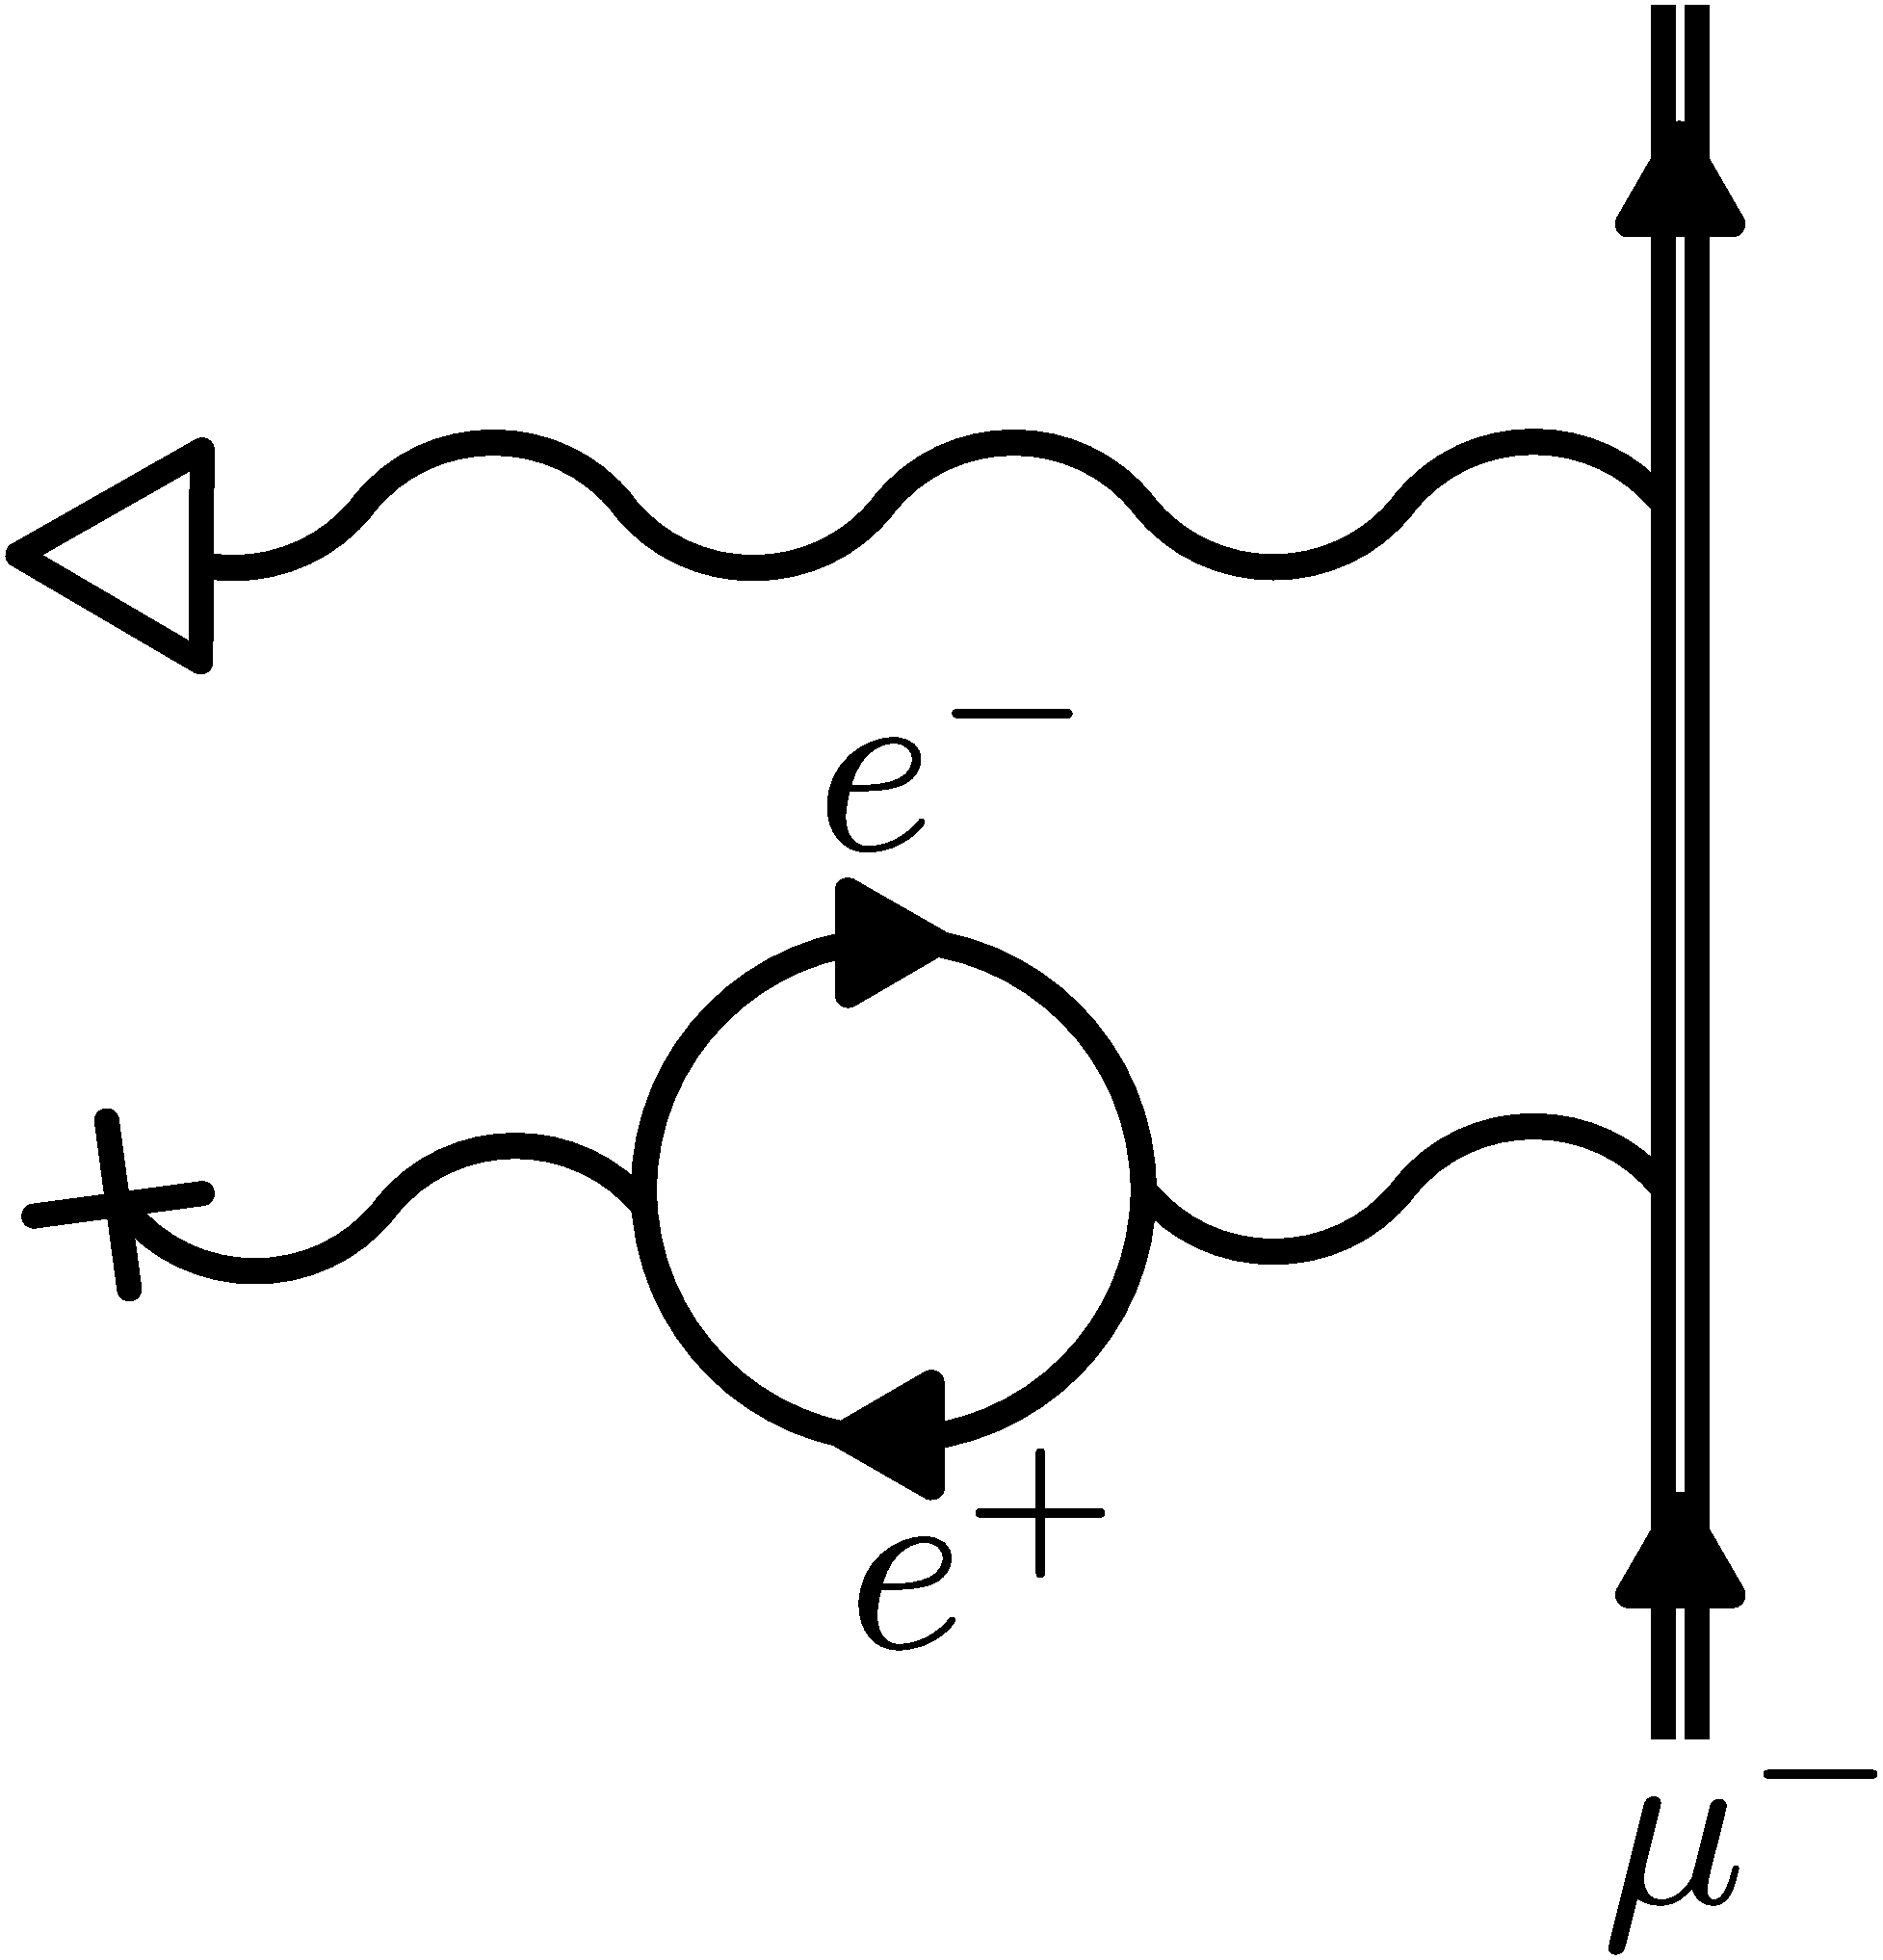
\includegraphics[width=0.22\textwidth]{pics/mixed}\hspace{3.5cm}
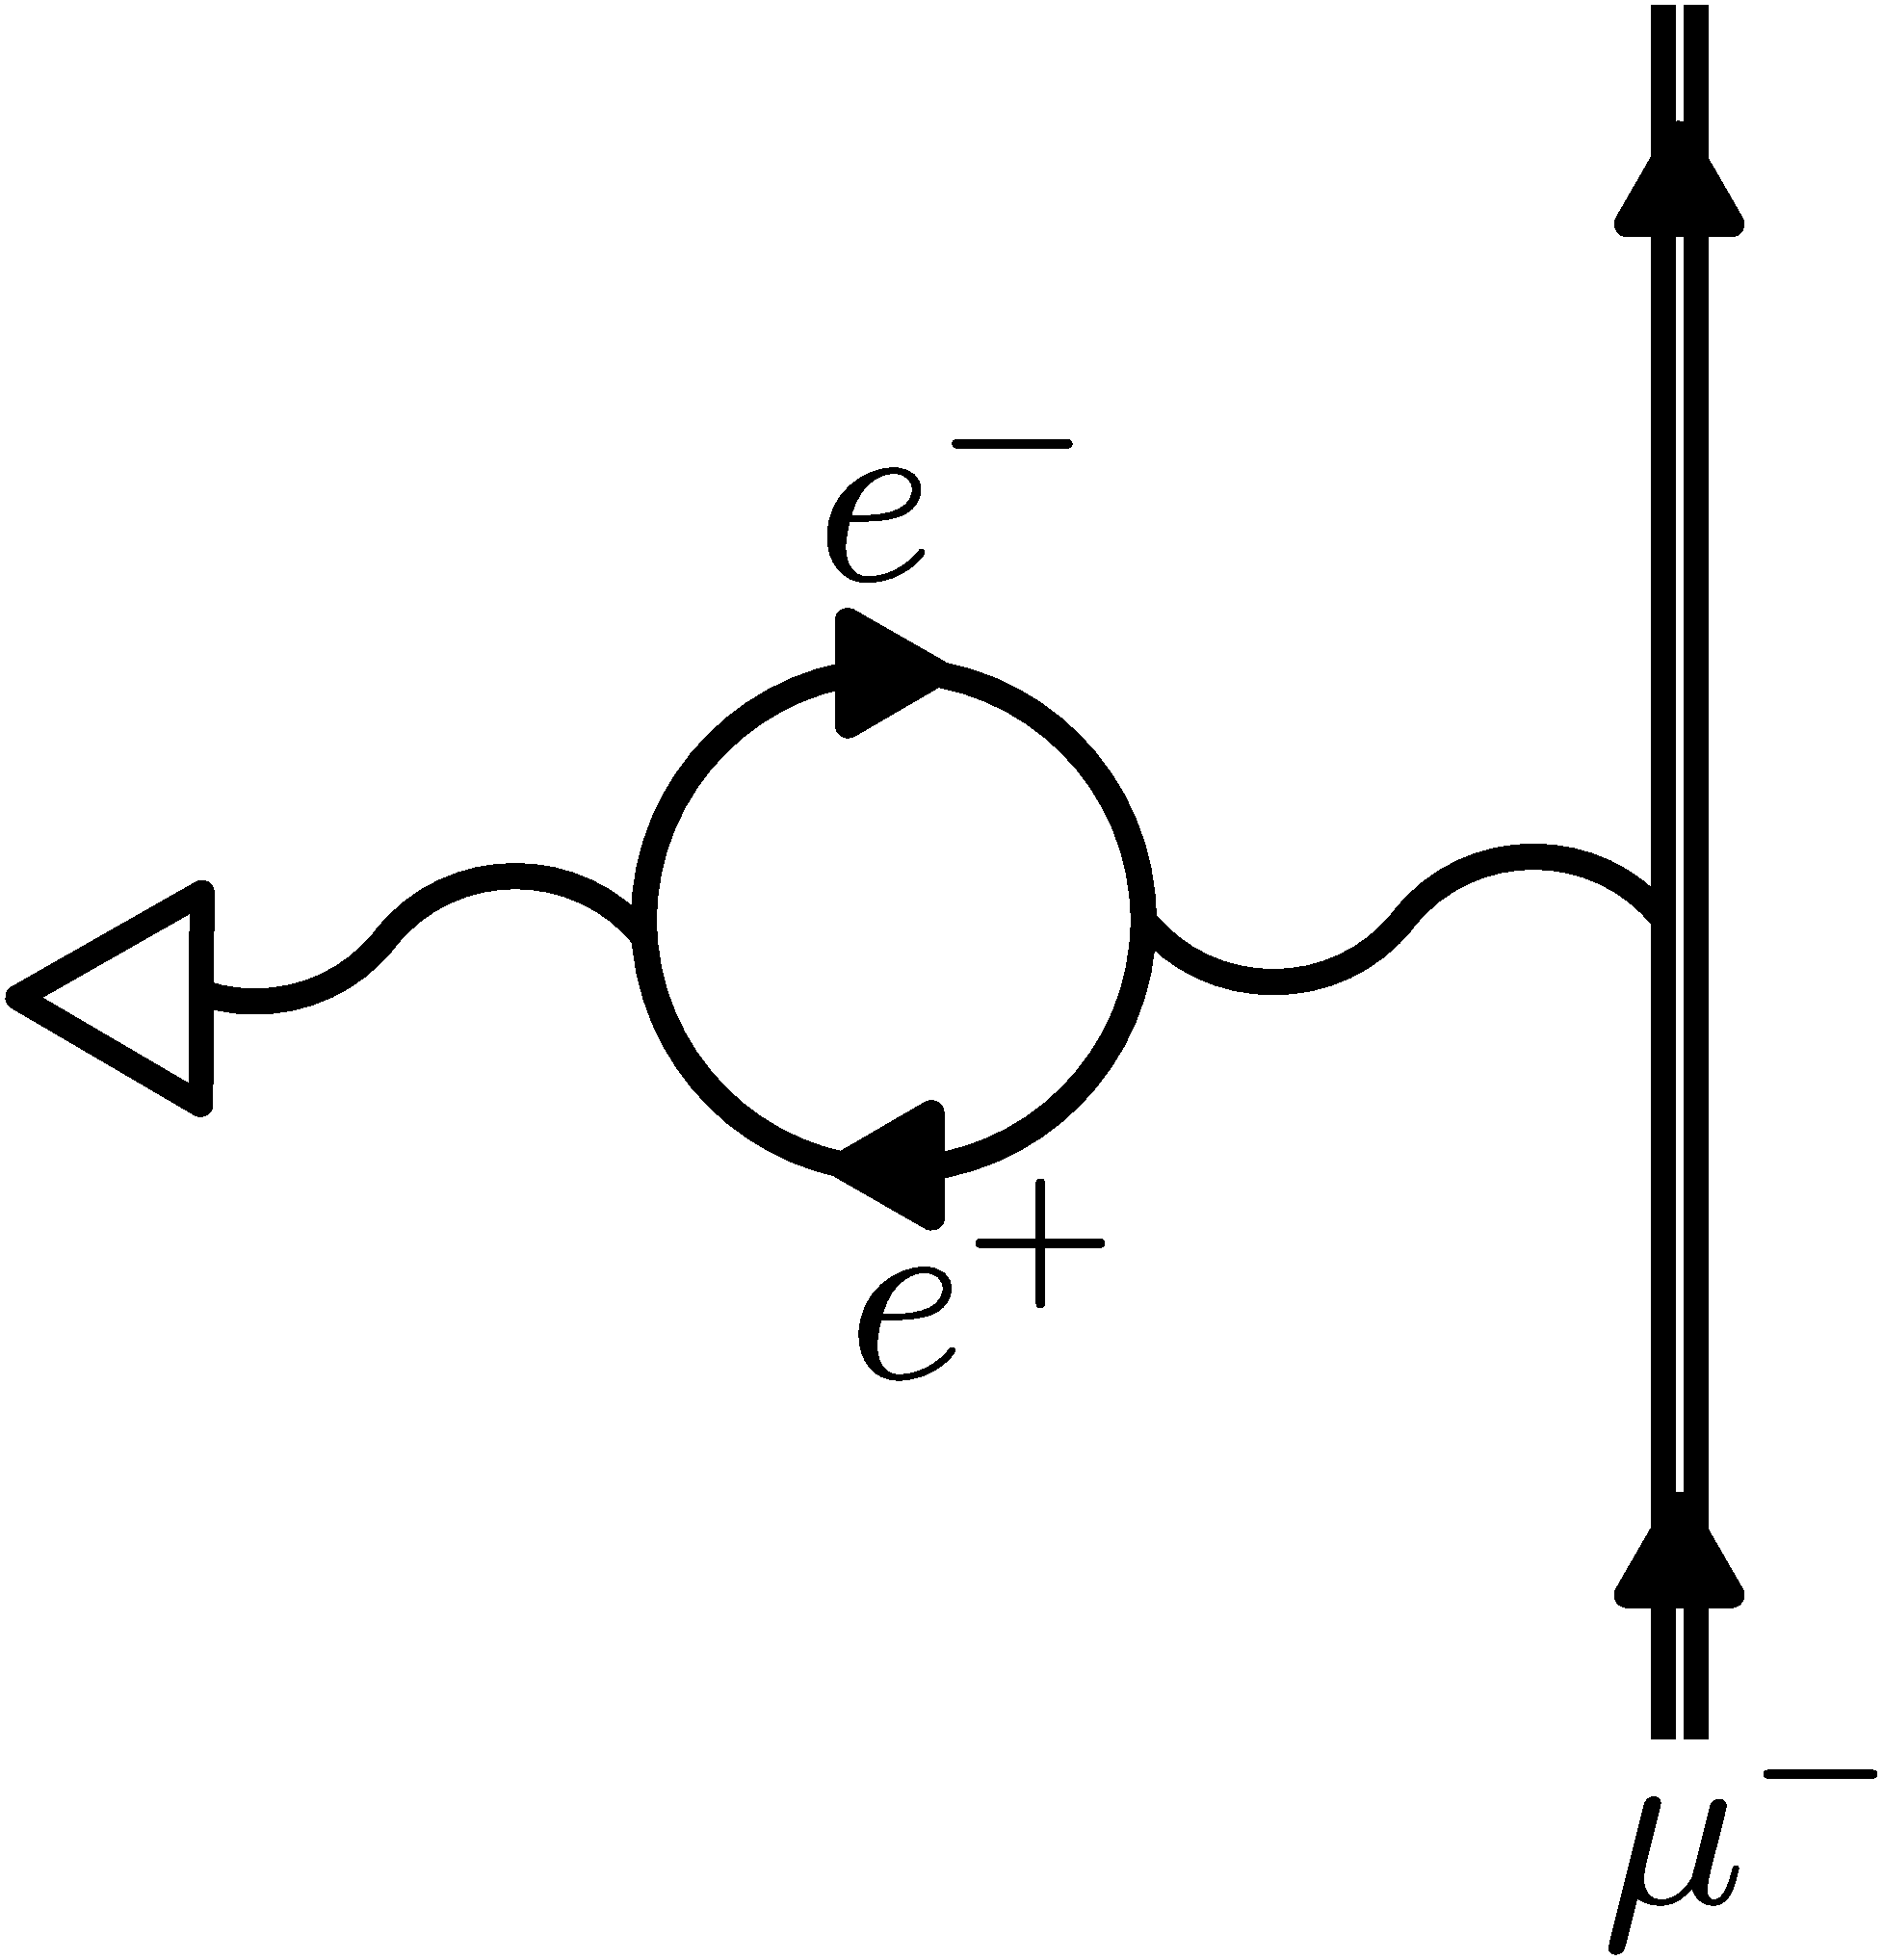
\includegraphics[width=0.22\textwidth]{pics/quehl}\\
$\qquad\qquad\qquad\qquad\qquad$(a)\hfill(b)$\qquad\qquad\qquad\qquad\qquad$
\caption{
Feynman diagrams for the leading order contributions of the vacuum polarization to the quadrupole interaction in muonic atoms. An external double line stands for the bound-muon wave function. A single internal line for the free electron propagator, and a wave line for the photon propagator. A cross represents the interaction with the monopole potential, and a triangle the interaction with the quadrupole potential. Contribution (a) is calculated by including the spherically symmetric contribution of the Uehling potential in the Dirac equation~\eqref{eq:h0mu}; Contribution (b) by including the quadrupole contribution of the Uehling potential in the matrix elements from Eq.~\eqref{eq:quadel_uehl} and \eqref{eq:second}.
}
\label{fig:quehl}
\end{figure}
%
%

The monopole terms $V^{(0)}_{\text{el}}(r_\mu)$ and $V^{(0)}_{\text{uehl}}(r_\mu)$ only depend on the muonic radial coordinate and thus were included in this work in the unperturbed muonic states as
\begin{equation}
\left( H_\mu + V^{(0)}_{\text{el}}+V^{(0)}_{\text{uehl}}\right) \left|n\kappa m\right> = E_{n\kappa}\left|n\kappa m \right>,
\label{eq:h0mu}
\end{equation}
where $\left|n\kappa m \right>$ are the solutions of the spherical Dirac equation in terms of the well-known spherical spinors and radial functions $G_{n\kappa}(r_\mu)$ and $F_{n\kappa}(r_\mu)$ with energy $E_{n \kappa}$~\cite{greiner2000}. $n$, $\kappa$, $m$ are the principal quantum number, the relativistic angular quantum number and the $z$ component of the total angular momentum of the muon, respectively. In this way, the monopole Uehling potential and all iterations thereof are included in the muonic wave functions~\cite{michel2017}.
\section{Electric quadrupole interaction}
\subsection{Dynamic Hyperfine structure}
The hyperfine splitting due to electric quadrupole interactions is considered in the coupled basis, where a state with total angular momentum $F$ and its projection on the $z$  axis $M$ is formed for a given muonic and nuclear state as
\begin{equation}
\left| FM\,n\kappa\,IK \right> = \sum_{m,M^\prime} C^{FM}_{jm\,IM^\prime} \left|n\kappa m\right>\otimes\left|IM^\prime K\right>,
\end{equation}
with the Clebsch-Gordan coefficients $C^{jm}_{j_1m_1\,j_2m_2}$. The matrix elements of the electric quadrupole interaction are written as
\begin{equation}
\Delta E^{(2)}_{\text{el}} = \left< FMn_1\kappa_1I_1K\right|{V_{\text{el}}^{(2)}}\left|FMn_2\kappa_2I_2K\right>,
\label{eq:quadel}
\end{equation}
where the diagonal elements correspond to the first order electric hyperfine splitting~\cite{michel2017}. The explicit expressions are given in Eqs.~\eqref{eq:matel} and~\eqref{eq:defmulti} in the Appendix.
\begin{table}[b]
\caption{\label{tab:params}%
Nuclear parameters used in the numerical calculations. $I_0$ is the nuclear ground state angular momentum. RMS and $Q_\text{spec}$ are the nuclear RMS radius and spectroscopic quadrupole moment of the nuclear ground state from~\cite{Angeli2013,Stone2005}, respectively. $c$, $a$, $\beta$ are the parameters of the deformed Fermi distribution derived from RMS and $Q_\text{spec}$, see Sec. \ref{sec:num} for details. $E_{I}$ are the excitation energies of the nuclear rotational states with angular momentum $I$ in Eq.~\eqref{eq:enucl}, the values are taken from~\cite{ENSDF}.}
%\begin{ruledtabular}
\centering
\begin{tabular}{rll}
& $^{185}_{\phantom{1}75}$Re & $^{235}_{\phantom{1}92}$U\\ \hline \\[-10pt]
$I_0$ \hfill$\phantom{.}$ & $5/2$ & $7/2$ \\
RMS \hfill[fm] & $5.3596(172)$ & $5.8337(41)$ \\
$Q_\text{spec}$ \hfill[b] & $2.21(4)\phantom{111}$ & $4.936(6)\phantom{1}$ \\
$c$ \hfill[fm] & $6.3517$ & $6.9562$ \\
$a$ \hfill[fm] & 0.5234 & 0.5234 \\
$\beta$ \hfill$\phantom{.abc.}$ & 0.2322 & 0.2711 \\[7pt]
$E_{I_0 + 1}$ \hfill[keV] & 125.3587(9) &  $\phantom{1}$46.108(8) \\
$E_{I_0 + 2}$ \hfill[keV] & 284.2(3) & 103.903(8) \\
$E_{I_0 + 3}$ \hfill[keV] & 475.7(4) & 171.464(13) \\
$E_{I_0 + 4}$ \hfill[keV] & 697.1(5) & 250.014(21) \\
$E_{I_0 + 5}$ \hfill[keV] & 949.7(5) & 339.976(24) \\
\end{tabular}
%\end{ruledtabular}
\end{table}
For heavy, deformed nuclei, the fine structure as well as the first order quadrupole hyperfine structure of muonic energy levels is similar to the energies of the low-lying nuclear rotational states. Therefore, the total Hamiltonian has to be rediagonalized in finite subspaces of a muonic finestructure multiplet and the first few nuclear rotational states. Since multipole interactions are diagonal in $F$ and $M$, there is no mixing of states with different total angular momentum. Thus, if $d$ is the dimension of the subspace, new states
\begin{equation}
\left| FM k \right> := \sum_{i=1}^{d} a^{(k)}_i \left| FM\,n_i\kappa_i\,I_iK \right>
\label{eq:compstate}
\end{equation}
with $k \in {1,...,d}$ may be defined, in which the coefficients $a_i^{(k)}$ have to be chosen such that the matrix representation of the total Hamiltonian \eqref{eq:htot} in the subspace is diagonal. The corresponding eigenenergies are written as $E^{(F,k)}_{\text{quad}}$. This leads to a rich and complex level structure and to hyperfine structure also for nuclei with zero ground-state angular momentum and is know as the dynamic hyperfine structure~\cite{wu1969,Devons1995}.

\subsection{Higher order contributions}
In this work, the VP in Uehling approximation is included in the dynamic hyperfine structure, considering the finite nuclear size. For this, the matrix elements of the quadrupole Uehling interaction
\begin{equation}
\Delta E^{(2)}_{\text{uehl}} = \left< FMn_1\kappa_1I_1K\right|{V_{\text{uehl}}^{(2)}}\left|FMn_2\kappa_2I_2K\right>,
\label{eq:quadel_uehl}
\end{equation}
are added to the matrix elements from Eq.~\eqref{eq:quadel}. The explicit formulas for Eq.~\eqref{eq:quadel_uehl} are given in Eqs.~\eqref{eq:matel} and~\eqref{eq:defmultiuehl} in the Appendix.
By including the monopole Uehling potential in the unperturbed muon states in Eq.~\eqref{eq:h0mu} and the quadrupole Uehling potential in the matrix elements~\eqref{eq:quadel_uehl}, all contributions of the Uehling potential to the electric quadrupole interactions are included, as shown schematically in Fig.~\ref{fig:quehl}~(a) and (b), respectively.

After a subspace has been chosen and rediagonalization has been performed, the quadrupole interaction with states outside of the subspace leads to residual second order corrections to the energy levels~\cite{chen1970}. 
For the total second order correction a summation over the complete (discrete and continous) spectrum for both nuclear and muonic states has to be performed. For the complete nuclear spectrum, sophisticated models or numerous experimental data are required. Therefore, in this work, we calculate the second order corrections, where the nucleus stays in the rotational ground state, but the complete muonic spectrum is considered.
The second order energy shift is
\begin{equation}
\Delta E_{\text{2.ord.}}^{(F,k)}= \sum_i\frac{\left|\left< FMk\right|{V_{\text{el}}^{(2)}}{+}{V_{\text{uehl}}^{(2)}}\left|FMn_i\kappa_iI_iK \right>\right|^2}{E_{F,k}-E_i},
\label{eq:second}
\end{equation}
where the sum is to be taken over all states not considered in the rediagonalization, including continuum states of the muon, and the unperturbed energy of the state $i$ is $E_i=E_{n_i\kappa_i}+E_{I_i}$.
%
%
\section{Numerical Evaluation}
\label{sec:num}
Calculations have been performed for muonic Rhenium and Uranium, assuming a deformed Fermi nuclear charge distribution which reads as
\begin{equation}
\rho_{ca\beta}(\vec{r}\,)=\cfrac{N}{1+\exp (\frac{r-c(1+\beta \text{Y}_{20}(\vartheta))}{a})},
\label{eq:deffermi_2}
\end{equation}
where $c$ is the half-density radius, $a$ the skin thickness, $\beta$ the deformation parameter, and $N$ a normalization constant determined by the condition
\begin{equation}
\int \text{d}^3r\, \rho_{ca\beta}(\vec{r}\,)=1.
\end{equation}
Using the deformed Fermi distribution has proved to be very successful in the description of the level structure of heavy muonic atoms, e.g.~\cite{hitlin1970,tanaka1984,tanaka1984_2}.
Values for the parameters can be estimated by using a value ${a}{=}{2.3\,\text{fm}/(4\ln 3)}$, which has proved to be a sufficiently accurate value for most nuclei~\cite{Beier2000}. Then, $c$ and $\beta$ are chosen such that the quadrupole moment and RMS value of the distribution are in agreement with the literature values from~\cite{Angeli2013,Stone2005}. For the nuclear states involved in the dynamic hyperfine structure, also the excitation energies are needed from literature~\cite{ENSDF}. The used parameters are summarized in Table~\ref{tab:params}.
With these parameters, the electric and Uehling potentials, both monopole and quadrupole parts, can be calculated numerically. The muon wave functions are obtained by solving the Dirac equation~\eqref{eq:h0mu} with the dual-kinetic-balance method~\cite{Shabaev2004}. Thereby, a complete set of muonic bound and continuum states is obtained. An overview for the binding energies of muon states important for the dynamic hyperfine splitting are shown in Table~\ref{tab:monopole}.

\begin{table}[b]
\caption{\label{tab:monopole}%
Binding energies of the low-lying, unperturbed muonic states due to the spherically symmetric parts of the electric and Uehling potential obtained by solving Eq.~\eqref{eq:h0mu} for muonic Rhenium and Uranium. The first column shows the binding energies for a point-like Coulomb potential, the second and third column include the finite size corrections without and with Uehling potential, respectively. See Sec. \ref{sec:num} for details. All energies are in keV.
}
%\begin{ruledtabular}
\centering
\begin{tabular}{ccrrr}
& state & \text{point like}& \text{finite size (fs)} &\text{fs+Uehling}\\ \hline \\[-7pt]
$^{185}$Re &1s\nicefrac{1}{2} & 17229.12 & 9333.46 & 9394.02 \\
&2s\nicefrac{1}{2} & 4398.85 & 3083.91 & 3100.44 \\
&2p\nicefrac{1}{2} & 4398.85 & 4032.61 & 4059.50 \\
&2p\nicefrac{3}{2} & 4033.07 & 3885.75 & 3910.50 \\
&3s\nicefrac{1}{2} & 1912.97 & 1498.01 & 1504.28 \\
&3p\nicefrac{1}{2} & 1912.97 & 1789.84 & 1798.66 \\
&3p\nicefrac{3}{2} & 1804.01 & 1751.38 & 1759.75 \\
&3d\nicefrac{3}{2} & 1804.01 & 1802.05 & 1810.30 \\
&3d\nicefrac{5}{2} & 1773.14 & 1772.36 & 1780.16 \\[7pt]
$^{235}$U&1s\nicefrac{1}{2} & 27351.29 & 12100.56 & 12175.51 \\
&2s\nicefrac{1}{2} & 7074.68 & 4308.67 & 4332.13 \\
&2p\nicefrac{1}{2} & 7074.68 & 5901.35 & 5941.39 \\
&2p\nicefrac{3}{2} & 6130.65 & 5674.78 & 5711.89 \\
&3s\nicefrac{1}{2} & 3033.18 & 2148.86 & 2158.31 \\
&3p\nicefrac{1}{2} & 3033.18 & 2645.58 & 2659.26 \\
&3p\nicefrac{3}{2} & 2751.54 & 2588.19 & 2601.27 \\
&3d\nicefrac{3}{2} & 2751.54 & 2739.69 & 2754.06 \\
&3d\nicefrac{5}{2} & 2679.66 & 2674.77 & 2688.10

\end{tabular}
%\end{ruledtabular}
\end{table}
%
%begin hfs table
\begin{table*}
\begin{small}
\caption{\label{tab:hfs_2}
Overview of energy corrections due to residual second order electric quadrupole splitting~$\Delta E_{\text{2.ord.}}$ and quadrupole-Uehling interaction~$\Delta E_{\text{quad-uehl}}$ for $^{185}$Re and $^{235}$U. $F$ is the total angular momentum of muon and nucleus, $I_N$ is the nuclear angular momentum and $\mu$-state is the muonic state in spectroscopic notation. For the muonic $2p$ and $3d$ states, these are mixed by the dynamic hyperfine structure, thus $I_N$ (main) and $\mu$-state (main) show the states with the largest contribution. $E_{\text{quad}}$ is the binding energy without quadrupole Uehling and residual second order quadrupole interaction, see Sec. \ref{sec:num} for details. The states are ordered descending in the total energy~$E_{\text{tot}}$. All energies are in keV.}
%\begin{ruledtabular}
\centering
\begin{tabular}{lrccccc|c}
 &F&\multicolumn{1}{c}{$I_{N}\,\text{(main)}$}&$\mu\text{-state (main)}$&\multicolumn{1}{c}{$E_{\text{quad}}$}&\multicolumn{1}{c}{$\Delta E_{\text{2.ord.}}$}&\multicolumn{1}{c}{$\Delta E_{\text{quad-uehl}}$}&\multicolumn{1}{c}{$E_{\text{tot}}$}\\\hline\\[-7pt]
$^{185}\text{Re}$&  2 &   \nicefrac{5}{2} & 1s\nicefrac{1}{2} & 9394.02 &  3.21 &   0.00 & 9397.23 \\
&  6 &  \nicefrac{13}{2} & 1s\nicefrac{1}{2} & 8696.92 &  2.06 &   0.00 & 8698.98 \\
&  8 &  \nicefrac{15}{2} & 1s\nicefrac{1}{2} & 8444.32 &  1.76 &   0.00 & 8446.08 \\
&  2 &   \nicefrac{5}{2} & 2p\nicefrac{1}{2} & 4083.31 &  2.18 &  0.28 & 4085.77 \\
&  3 &   \nicefrac{5}{2} & 2p\nicefrac{1}{2} & 4077.79 &  2.07 &  0.23 & 4080.09 \\
&  3 &   \nicefrac{9}{2} & 2p\nicefrac{3}{2} & 3992.27 &  2.41 &  0.41 & 3995.09 \\
&  4 &   \nicefrac{7}{2} & 2p\nicefrac{1}{2} & 3957.33 &  2.10 &  0.26 & 3959.69 \\
&  3 &   \nicefrac{5}{2} & 2p\nicefrac{3}{2} & 3886.35 &  1.12 & -0.22 & 3887.25 \\
&  5 &   \nicefrac{7}{2} & 2p\nicefrac{3}{2} & 3814.27 &  2.08 &  0.28 & 3816.63 \\
&  4 &   \nicefrac{9}{2} & 2p\nicefrac{1}{2} & 3734.93 &  1.03 & -0.27 & 3735.69 \\
&  6 &   \nicefrac{9}{2} & 2p\nicefrac{3}{2} & 3650.57 &  1.95 &  0.25 & 3652.77 \\
&  5 &   \nicefrac{9}{2} & 2p\nicefrac{3}{2} & 3556.36 &  1.13 & -0.24 & 3557.25 \\
&  7 &  \nicefrac{11}{2} & 2p\nicefrac{3}{2} & 3458.14 &  1.85 &  0.23 & 3460.22 \\
&  6 &  \nicefrac{11}{2} & 2p\nicefrac{3}{2} & 3344.35 &  0.93 & -0.19 & 3345.09 \\
&  8 &  \nicefrac{13}{2} & 2p\nicefrac{3}{2} & 3111.03 &  0.68 &  0.02 & 3111.73 \\
&  7 &  \nicefrac{15}{2} & 2p\nicefrac{3}{2} & 2941.66 &  0.82 & -0.15 & 2942.33 \\
&  8 &  \nicefrac{15}{2} & 2p\nicefrac{3}{2} & 2938.52 &  0.67 & -0.16 & 2939.03 \\
&  3 &   \nicefrac{5}{2} & 3d\nicefrac{3}{2} & 1815.47 &  0.07 &  0.03 & 1815.57 \\
&  1 &   \nicefrac{5}{2} & 3d\nicefrac{3}{2} & 1804.28 &  0.11 & -0.03 & 1804.36 \\
&  3 &   \nicefrac{7}{2} & 3d\nicefrac{5}{2} & 1783.72 &  0.05 &  0.02 & 1783.79 \\
&  0 &   \nicefrac{5}{2} & 3d\nicefrac{5}{2} & 1772.11 &  0.11 & -0.04 & 1772.18 \\[7pt]
$^{235}\text{U}$&  3 &   \nicefrac{7}{2} & 1s\nicefrac{1}{2} & 12175.51 &  6.83 &   0.00 & 12182.34 \\
&  7 &  \nicefrac{15}{2} & 1s\nicefrac{1}{2} & 11925.50&  4.66 &  0.00  & 11930.16 \\
&  9 &  \nicefrac{17}{2} & 1s\nicefrac{1}{2} & 11835.54&  3.54 &  0.00  & 11839.08 \\
&  3 &   \nicefrac{7}{2} & 2p\nicefrac{1}{2} & 6019.06 &  5.99 &  0.85 & 6025.90 \\
&  4 &   \nicefrac{7}{2} & 2p\nicefrac{1}{2} & 6015.01 &  5.96 &  0.83 & 6021.80 \\
&  4 &   \nicefrac{9}{2} & 2p\nicefrac{1}{2} & 5979.31 &  6.02 &  0.86 & 5986.19 \\
&  5 &   \nicefrac{9}{2} & 2p\nicefrac{3}{2} & 5928.94 &  6.06 &  0.88 & 5935.88 \\
&  6 &  \nicefrac{11}{2} & 2p\nicefrac{3}{2} & 5868.85 &  6.00 &  0.89 & 5875.74 \\
&  7 &  \nicefrac{15}{2} & 2p\nicefrac{1}{2} & 5798.66 &  5.30 &  0.91 & 5804.87 \\
&  8 &  \nicefrac{15}{2} & 2p\nicefrac{1}{2} & 5745.59 &  4.71 &  0.87 & 5751.17 \\
&  5 &   \nicefrac{7}{2} & 2p\nicefrac{3}{2} & 5673.10 &  3.12 & -0.42 & 5675.80 \\
&  6 &   \nicefrac{9}{2} & 2p\nicefrac{3}{2} & 5621.02 &  3.02 & -0.46 & 5623.58 \\
&  2 &   \nicefrac{7}{2} & 2p\nicefrac{3}{2} & 5620.12 &  2.78 & -0.56 & 5622.34 \\
&  9 &  \nicefrac{17}{2} & 2p\nicefrac{1}{2} & 5613.24 &  2.05 &  0.13 & 5615.42 \\
&  3 &   \nicefrac{9}{2} & 2p\nicefrac{3}{2} & 5586.28 &  2.81 & -0.54 & 5588.55 \\
&  7 &  \nicefrac{13}{2} & 2p\nicefrac{1}{2} & 5556.38 &  2.60 & -0.50 & 5558.48 \\
&  9 &  \nicefrac{15}{2} & 2p\nicefrac{3}{2} & 5493.59 &  2.44 &  0.24 & 5496.27 \\
&  8 &  \nicefrac{15}{2} & 2p\nicefrac{1}{2} & 5479.30 &  2.14 & -0.53 & 5480.91 \\
& 10 &  \nicefrac{17}{2} & 2p\nicefrac{3}{2} & 5393.16 &  1.77 &  0.13 & 5395.06 \\
&  9 &  \nicefrac{17}{2} & 2p\nicefrac{3}{2} & 5315.81 &  1.73 & -0.44 & 5317.10 \\
&  3 &   \nicefrac{7}{2} & 3d\nicefrac{3}{2} & 2767.16 &  0.44 &  0.09 & 2767.69 \\
&  1 &   \nicefrac{7}{2} & 3d\nicefrac{5}{2} & 2663.35 &  0.61 & -0.13 & 2663.83 \\
\end{tabular}
%\end{ruledtabular}
\end{small}
\end{table*}
% end hfs table
The quadrupole matrix elements from Eq.~\eqref{eq:quadel} can be calculated both for the rediagonalization in the dynamic hyperfine structure and for the evaluation of the residual second-order terms \eqref{eq:second}, using Eq.~\eqref{eq:matel}. As the next step, the total Hamiltonian~\eqref{eq:htot} is diagonalized in finite subspaces or modelspaces consisting of the muonic ($2p\nicefrac{1}{2}$, $2p\nicefrac{3}{2}$) or ($3d\nicefrac{3}{2}$, $3d\nicefrac{5}{2}$) doublet states and nuclear ground state rotational band. For Rhenium, the first six states with $I_N \in \{5/2,...,15/2\}$ are considered, and for Uranium with $I_N \in \{7/2,...,17/2\}$. The excitation energies of the nuclear states are summarized, along with other nuclear parameters, in Table~\ref{tab:params}. Thereby, the composite states and corresponding energies $E_{\text{quad}}$ from Eq.~\eqref{eq:compstate} are obtained and finally, for each of these states the residual second order quadrupole correction \eqref{eq:second} is calculated. Here, the intermediate sum goes over all nuclear and muonic states not included in the modelspace.
Note that for the muonic ground state, a rediagonalization is not necessary, since the diagonal matrix elements of the quadrupole interactions vanish for muonic states with $j=1/2$.
The quadrupole-Uehling contribution to the binding energies can be obtained by performing the calculations for the dynamic hyperfine structure twice; once with the matrix elements~\eqref{eq:quadel} and~\eqref{eq:quadel_uehl} containing both the electric and Uehling interaction ${V_{\text{el}}^{(2)}}{+}{V_{\text{uehl}}^{(2)}}$ and a second time only with the electric part ${V_{\text{el}}^{(2)}}$ from Eq.\eqref{eq:quadel}. The difference between those two approaches gives the quadrupole-Uehling corrections. Results for the residual second order quadrupole correction from Eq.~\eqref{eq:second} and for the quadrupole-Uehling corrections can be found in Table~\ref{tab:hfs_2} for a number of states.
\section{Discussion and Summary}
The quadrupole interaction in the framework of the dynamic hyperfine structure in heavy muonic atoms was analyzed by an fully relativistic treatment of the quadrupole-Uehling potential and of the residual second order terms.
The quadrupole-Uehling interaction was obtained by a multipole expansion of the Uehling potential for an arbitrary nuclear charge distribution without the assumption on the distance between muon and nuclear charge being large.
Since it has the same angular structure as the conventional quadrupole interaction, the quadrupole-Uehling expectation value vanishes between two muonic states with $j=1/2$, thus it does not affect the muonic ground state.
The calculations for Uranium show that it can lead to energy corrections almost on the keV level for very heavy nuclei with muonic $2p$ states and thus can be potentially relevant for comparison between theoretical predictions and experiments. Being a short-ranged potential, it falls of quickly for states further away from the nucleus. For states with $n\geq3$, we find values below $0.15\,$keV, even for high Z.
The generalization to Uehling corrections for higher order multipole is straight forward. In the case of muonic atoms, since the influence of higher order multipoles is already small, we expect this correction will not contribute significantly.

The residual second order quadrupole corrections in the dynamic hyperfine structure were calculated numerically using a basis of relativistic wave functions including nuclear finite size correction and Uehling correction due to the monopole part of the nuclear potential.
In contrast to the first order terms, the muonic ground state energy is affected by the second order corrections. Here, the energy correction amounts up to several keV. Also for muonic $2p$ states, it is of similar size. For the $3d$ levels, we find the energy corrections below half a keV, both for Rhenium and Uranium.
If a more complete nuclear model instead the rotational model is used, the additional nuclear states appear as intermediate state in the second order corrections, leading to the nuclear polarization corrections. Therefore, the approach presented in this work provides a basis for an accurate treatment of the muonic spectrum for the nuclear polarization effect in deformed muonic atoms.

\section{Multipole expansion of electric \\and Uehling potential}
\label{sec:multipole}
With the multipole expansion of the Coulomb potential~\cite{jackson1999}
\begin{equation}
\frac{1}{|\vec{r}_\mu^{\,\prime}-\vec{r}_N^{\,\prime}|}=\sum_{l=0}^\infty \frac{r_<^l}{r_>^{l+1}}\sum_{m=-l}^l  \text{C}^*_{lm}(\vartheta_N^{\prime},\varphi_N^{\prime})\text{C}_{lm}(\vartheta_\mu^\prime,\varphi_\mu^\prime),
\end{equation}
where $r_<:=\min (r_\mu,r_N)$, $r_>:=\max (r_\mu,r_N)$, the electric potential~\eqref{eq:pot} can be written as
\begin{align}
V_{\text{el}}(\vec{r}_\mu^{\,\prime})=&\sum_{l,m}-Z\alpha \left[ \int \text{d}^3r^{\prime}_N \frac{r_<^l}{r_>^{l+1}}\text{C}^*_{lm}(\vartheta_N^{\prime},\varphi_N^{\prime})\rho(\vec{r}_N^{\,\prime})\right]\notag\\
&\,\times\text{C}_{lm}(\vartheta_\mu^{\prime},\varphi_\mu^\prime),
\end{align}
where ${\text{C}_{lm}(\vartheta,\varphi)}{=}{\sqrt{4\pi/(2l+1)}\text{Y}_{lm}(\vartheta,\varphi)}$ are the normalized spherical harmonics and primed coordinates belong to the nuclear body-fixed system.
For axially symmetric charge distributions, only the ${m}{=}{0}$-terms are non-zero after integrating over the charge distribution. The dependency on the muonic angular variables can be transformed to the laboratory system by
\begin{equation}
\text{P}_{l}(\cos\vartheta_\mu^\prime)=
 \sum_{m=-l}^l C^*_{lm}(\theta,\phi)C_{lm}(\vartheta_\mu,\varphi_\mu).
\end{equation}
Thereby, the potential as a function of the Euler angles and the muon's position in the laboratory frame reads
\begin{align}
V_{\text{el}}(\vec{r}_\mu,\phi,\theta)=&\sum_{l=0}^\infty-Z\alpha \left[ \int \text{d}^3r^{\prime}_N \frac{r_<^l}{r_>^{l+1}}\text{P}_{l}(\cos \vartheta_N^{\prime})\rho(\vec{r}_N^{\,\prime})\right]\notag\\
&\quad\,\times \sum_{m=-l}^l \text{C}^*_{lm}(\theta,\phi)\text{C}_{lm}(\vartheta_\mu,\varphi_\mu).\notag\\
=:&\sum_{l=0}^\infty Q_{\text{el}}^{(l)}(r_\mu)\sum_{m=-l}^lC^*_{lm}(\theta,\phi)C_{lm}(\vartheta_\mu,\varphi_\mu)&\notag\\
=:& \sum_{l=0}^\infty V^{(l)}_{\text{el}}(\vec{r}_\mu,\phi,\theta),
\label{eq:defmulti}
\end{align}
where $Q_{\text{el}}^{(l)}(r_\mu)$ describe the radial distribution of the mulitpole moments.

The Uehling potential can be expanded in multipoles in a similar way, now with a different dependence on $|\vec{r}_\mu^{\,\prime}-\vec{r}_N^{\,\prime}|$, as
\begin{align}
\frac{K_1(2m_e{|\vec{r}_\mu^{\,\prime} - \vec{r}^{\,\prime}\,|})}{|\vec{r}_\mu^{\,\prime} - \vec{r}^{\,\prime}\,|}
&=\sum_{l=0}^\infty c_l(r_\mu,r_N)\\
&\times\sum_{m=-l}^l \text{C}^*_{lm}(\vartheta_N^{\prime},\varphi_N^{\prime})\text{C}_{lm}(\vartheta_\mu^\prime,\varphi_\mu^\prime).\notag
\end{align}
The expansion coefficients $c_l$ can be calculated, using the fact that rotations do not change the absolute value of vectors, as
\begin{equation}
|\vec{r}_\mu^{\,\prime} - \vec{r}_N^{\,\prime}|
=|\vec{r}_\mu - \vec{r}_N|
=\sqrt{r_\mu^2 + r_N^2 - 2 r_\mu r_N y},
\end{equation}
with ${y}{=}{\cos(\sphericalangle \vec{r}_\mu\vec{r}_N)}$ being the cosine of the angle between the vectors $\vec{r}_\mu$ and $\vec{r}_N$, and read as
\begin{equation}
c_l(r_\mu,r_N)=\frac{2l+1}{2} \int_{-1}^1 \text{d}y \frac{K_1(2m_e{|\vec{r}_\mu - \vec{r}_N|})}{|\vec{r}_\mu - \vec{r}_N|} P_l(y),
\label{eq:defcl}
\end{equation}
and are evaluated by numerical integration.
Thereby, the Uehling potential can be written, analogously to Eq.~\eqref{eq:defmulti}, as
\begin{align}
V_{\text{uehl}}(\vec{r}_\mu,\phi,\theta)=&\sum_{l=0}^\infty-Z\alpha\frac{2\alpha}{3\pi} \notag\\
&\quad\times\left[ \int \text{d}^3r^{\prime}_N c_l(r_\mu,r_N)\text{P}_{l}(\cos \vartheta_N^{\prime})\rho(\vec{r}_N^{\,\prime})\right]\notag\\
&\quad\,\times \sum_{m=-l}^l \text{C}^*_{lm}(\theta,\phi)\text{C}_{lm}(\vartheta_\mu,\varphi_\mu).\notag\\
=:&\sum_{l=0}^\infty Q^{(l)}_{\text{uehl}}(r_\mu)\times\sum_{m=-l}^lC^*_{lm}(\theta,\phi)C_{lm}(\vartheta_\mu,\varphi_\mu)&\notag\\
=:& \sum_{l=0}^\infty V^{(l)}_{\text{uehl}}(\vec{r}_\mu,\phi,\theta).
\label{eq:defmultiuehl}
\end{align}
For $l=0$, the expression for Uehling potential of a spherical charge distribution~\cite{Fullerton1976} which only depends on $r_\mu$ is recovered as
\begin{align}
\label{eq:sph_uehl}
V^{(0)}_{\text{uehl}}(r_\mu)=& -\frac{2\alpha (Z\alpha)}{3 m_e r}\int_0^\infty \text{d}r^{\prime}\,\rho_0(r^\prime)\\
&\times\left[K_0(2m_e|r-r^\prime|)-K_0(2m_e(r+r^\prime))\right]\notag
\end{align}
where the spherically averaged part of the charge distribution is
\begin{equation}
\rho_0(r)=\int_0^{2\pi}\text{d}\varphi\int_0^\pi\text{d}\vartheta \sin(\vartheta)\rho(\vec{r}\,)/(4\pi).
\end{equation}
%
%
\section{Matrix elements of quadrupole interactions}
\label{sec:mat}
Both the electric and Uehling multipole interaction are a scalar product of rank-$l$ spherical tensors in the angular variables of the muon and of the nucleus. Thus, their matrix elements in states of defined total angular momentum can be reduced to a product of two reduced matrix elements~\cite{varshalovich1988} as
\begin{align}
&{\left< F_1M_1n_1\kappa_1I_1K\right|V^{(l)}(\vec{r}_\mu,\phi,\theta)\left|FMn_2\kappa_2I_2K\right>} {=}
{\delta_{\scriptscriptstyle F_1F_2}\delta_{\scriptscriptstyle M_1M_2}}\notag\\
&\qquad\times(-1)^{F_1+j_2+I_1}
\left\{
\begin{matrix}
j_1&j_2&l\\
I_1&I_2&F_1
\end{matrix}
\right\}\left< I_1K\big{|}\big{|}\text{C}_l(\theta,\phi)\big{|}\big{|}I_2K\right>\notag\\
&\qquad\times \left< n_1\kappa_1\big{|}\big{|}Q^{(l)}(r_\mu)\text{C}_l(\vartheta_\mu,\varphi_\mu) \big{|}\big{|}n_2\kappa_2\right>.\label{eq:matel}
\end{align}
The matrix elements for the nucleus, reduced in $M$ but not in $K$, read~\cite{brown_carrington}
\begin{align}
\left< I_1K\big{|}\big{|}\text{C}_l(\theta,\phi)\big{|}\big{|}I_2K\right>=&(-1)^{I_2+K}
\sqrt{(2I_1+1)(2I_2+1)}\notag\\
&\times\,\left(
\begin{matrix}
I_1&I_2&l\\
-K&K&0
\end{matrix}
\right),
\end{align}
and the reduced matrix elements in the muonic variables are~\cite{johnson2007}
\begin{align}
&\left< n_1\kappa_1\big{|}\big{|}Q^{(l)}(r_\mu)\text{C}_l(\vartheta_\mu,\varphi_\mu) \big{|}\big{|}n_2\kappa_2\right> =  \\
&\quad (-1)^{j_1+1/2} \sqrt{(2j_1+1)(2j_2+1)}
\left(
\begin{matrix}
j_1&j_2&l\\
-\frac{1}{2}&\frac{1}{2}&0
\end{matrix}
\right)\notag\\
&\quad\times\,
\int \text{d}rr^2 ({g_{n_1\kappa_1}(r)g_{n_2\kappa_2}(r)}{+}{f_{n_1\kappa_1}(r)f_{n_2\kappa_2}(r)}) Q^{(l)}(r_\mu),\notag
\end{align}
where $g_{n\kappa}(r)$ and $f_{n\kappa}(r)$ are the two radial functions of the solutions of the Dirac equation in the spherically symmetric potential~\cite{greiner2000} from Eq.~\eqref{eq:h0mu}.






